% ============================================================================
% SLIDE BẢO VỆ LUẬN VĂN THẠC SĨ
% Mạng Đối Nghịch Tạo Sinh Trong Chuyển Đổi Ảnh Chân Dung Sang Phong Cách Anime
% Nguyễn Trọng Nhân - 24025149
% ============================================================================

\documentclass[aspectratio=169,12pt]{beamer}

% === PACKAGES ===
\usepackage[utf8]{inputenc}
\usepackage[vietnamese]{babel}
\usepackage{graphicx}
\usepackage{booktabs}
\usepackage{amsmath,amssymb}
\usepackage{tikz}
\usepackage{xcolor}
\usepackage{hyperref}
\usepackage{multicol}
\usepackage{array}
\usepackage{colortbl}
\usepackage{fontspec}
\usepackage{caption}

% === THEME CONFIGURATION ===
\usetheme{Madrid}
\usecolortheme{whale}

% Custom UET colors
\definecolor{uetblue}{RGB}{0, 51, 102}
\definecolor{uetgold}{RGB}{204, 153, 0}
\definecolor{uetred}{RGB}{180, 0, 0}
\definecolor{lightblue}{RGB}{230, 240, 255}
\definecolor{darkblue}{RGB}{0, 40, 85}
\definecolor{resultgreen}{RGB}{0, 128, 0}
\definecolor{slidebg}{RGB}{245, 248, 252}

\setbeamercolor{structure}{fg=uetblue}
\setbeamercolor{palette primary}{bg=uetblue, fg=white}
\setbeamercolor{palette secondary}{bg=uetblue!80, fg=white}
\setbeamercolor{palette tertiary}{bg=uetblue!60, fg=white}
\setbeamercolor{frametitle}{bg=uetblue, fg=white}
\setbeamercolor{title}{fg=white, bg=uetblue}
\setbeamercolor{block title}{bg=uetblue, fg=white}
\setbeamercolor{block body}{bg=lightblue, fg=black}
\setbeamercolor{block title alerted}{bg=uetred, fg=white}
\setbeamercolor{block body alerted}{bg=uetred!10, fg=black}
\setbeamercolor{block title example}{bg=resultgreen!80, fg=white}
\setbeamercolor{block body example}{bg=resultgreen!10, fg=black}
\setbeamercolor{item}{fg=uetblue}
\setbeamercolor{footline}{bg=uetblue!90, fg=white}

% Font settings
\setbeamerfont{title}{size=\Large, series=\bfseries}
\setbeamerfont{frametitle}{size=\large, series=\bfseries}
\setbeamerfont{footnote}{size=\tiny}

% Remove navigation symbols
\setbeamertemplate{navigation symbols}{}

% Custom footline
\setbeamertemplate{footline}{
  \leavevmode%
  \hbox{%
  \begin{beamercolorbox}[wd=.33\paperwidth,ht=2.5ex,dp=1ex,center]{footline}%
    \usebeamerfont{author in head/foot}\insertshortauthor
  \end{beamercolorbox}%
  \begin{beamercolorbox}[wd=.44\paperwidth,ht=2.5ex,dp=1ex,center]{footline}%
    \usebeamerfont{title in head/foot}\insertshorttitle
  \end{beamercolorbox}%
  \begin{beamercolorbox}[wd=.23\paperwidth,ht=2.5ex,dp=1ex,right]{footline}%
    \usebeamerfont{date in head/foot}\insertframenumber{} / \inserttotalframenumber\hspace*{2ex}
  \end{beamercolorbox}}%
}

% === METADATA ===
\title[GAN cho Anime hóa ảnh chân dung]{Mạng Đối Nghịch Tạo Sinh Trong Chuyển Đổi \\ Ảnh Chân Dung Sang Phong Cách Anime}
\subtitle{Luận văn Thạc sĩ Khoa học Máy tính}
\author[Nguyễn Trọng Nhân]{Học viên: \textbf{Nguyễn Trọng Nhân} \\ Mã HV: 24025149 \\ Giáo viên hướng dẫn: \textbf{TS. Ma Thị Châu}}
\institute[UET-VNU]{Trường Đại học Công nghệ \\ Đại học Quốc gia Hà Nội}
\date{Hà Nội, 2026}

% ============================================================================
\begin{document}

% ============================================================================
% SLIDE 1: TITLE PAGE
% ============================================================================
{
\setbeamertemplate{footline}{}
\begin{frame}
\vspace{-0.3cm}
\begin{columns}
\begin{column}{0.15\textwidth}
\centering

\includegraphics[width=0.9\linewidth]{figures/UET_logo.jpg}
\end{column}
\begin{column}{0.85\textwidth}
\centering
{\small ĐẠI HỌC QUỐC GIA HÀ NỘI}\\
{\small \textbf{TRƯỜNG ĐẠI HỌC CÔNG NGHỆ}}
\end{column}
\end{columns}
\vspace{0.3cm}
\titlepage
\end{frame}
}

% ============================================================================
% SLIDE 2: NỘI DUNG TRÌNH BÀY
% ============================================================================
\begin{frame}{Nội dung trình bày}
\tableofcontents[hideallsubsections]
\end{frame}

% ============================================================================
% PHẦN MỞ ĐẦU
% ============================================================================
\section{Mở đầu}

% --- Slide: Tính cấp thiết ---
\begin{frame}{Tính cấp thiết và ý nghĩa của đề tài}
\begin{columns}[T]
\begin{column}{0.55\textwidth}
\begin{itemize}
    \item Thị trường anime toàn cầu \textbf{81,96 tỷ USD} (2024), dự kiến $>$200 tỷ USD (2034)
    \item Nhu cầu tự động hóa chuyển đổi ảnh thực $\to$ phong cách anime
    \item \textbf{Thách thức:}
    \begin{itemize}
        \item Phong cách anime rất khác biệt ảnh thực
        \item Neural Style Transfer gặp nhiễu, artifacts
        \item CycleGAN chậm, chất lượng chưa ổn định
    \end{itemize}
    \item \textbf{GAN} nổi lên như giải pháp đột phá
\end{itemize}
\end{column}
\begin{column}{0.42\textwidth}
\centering
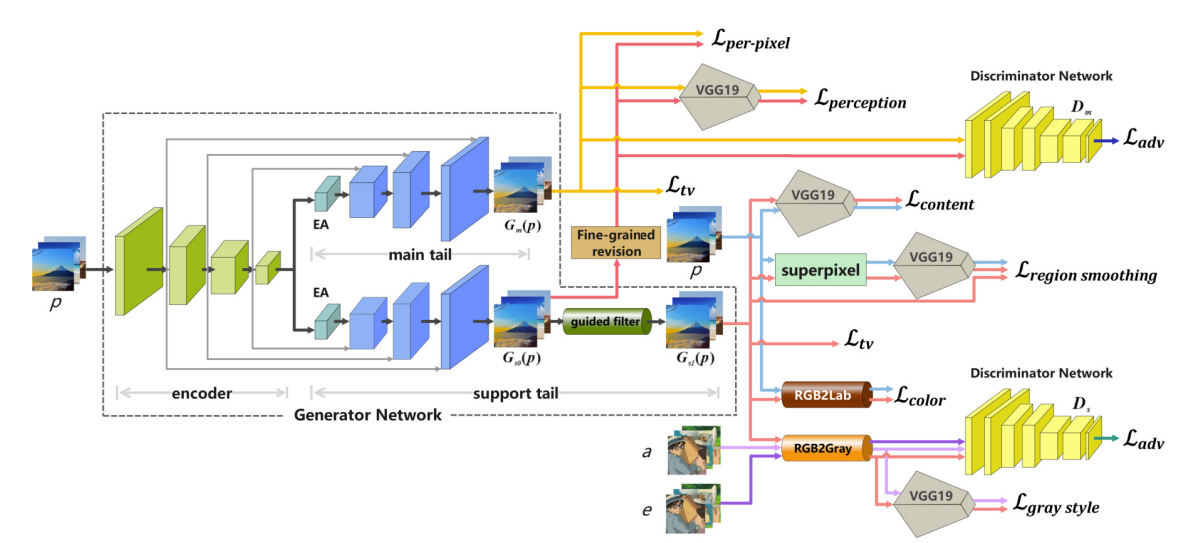
\includegraphics[width=\textwidth]{figChap1/pipelineDTGan.png}\\
{\scriptsize Sơ đồ tổng quát DTGAN}
\end{column}
\end{columns}
\end{frame}

% --- Slide: Mục tiêu nghiên cứu ---
\begin{frame}{Mục tiêu nghiên cứu}
\begin{enumerate}
    \item \textbf{Nghiên cứu nền tảng lý thuyết} CNN, GAN và các biến thể, kỹ thuật phát hiện khuôn mặt
    \item \textbf{Phân tích kiến trúc AnimeGANv3 (DTGAN)}: Double-Tail Generator, LADE, External Attention v3, hệ thống hàm mất mát
    \item \textbf{Xây dựng module Face Extraction} tích hợp RetinaFace + Margin Expansion $\to$ Pipeline end-to-end
    \item \textbf{Huấn luyện và đánh giá} trên phong cách Hayao Miyazaki, Makoto Shinkai (FID, LPIPS, FPS)
    \item \textbf{Triển khai ứng dụng web} (React + FastAPI) suy luận qua ONNX Runtime
\end{enumerate}
\end{frame}

% ============================================================================
% CHƯƠNG 1
% ============================================================================
\section{Cơ sở lý thuyết}

% --- Slide: Bài toán ---
\begin{frame}{Bài toán chuyển ảnh sang phong cách Anime}
\begin{block}{Định nghĩa}
Cho ảnh thực $x \in \mathcal{X}$, tìm ánh xạ $G: \mathcal{X} \to \mathcal{Y}$ sao cho $G(x)$ mang phong cách anime nhưng \textbf{bảo toàn nội dung} ảnh gốc. Dữ liệu huấn luyện \textbf{không ghép cặp} (unpaired).
\end{block}

\begin{columns}[T]
\begin{column}{0.48\textwidth}
\textbf{Đặc trưng phong cách anime:}
\begin{itemize}
    \item Đường nét viền rõ ràng (ink outline)
    \item Vùng màu phẳng (cel-shading)
    \item Đơn giản hóa chi tiết texture
    \item Màu sắc tươi sáng, bão hòa
\end{itemize}
\end{column}
\begin{column}{0.48\textwidth}
\textbf{Thách thức kỹ thuật:}
\begin{itemize}
    \item Cân bằng nội dung vs. phong cách
    \item Dữ liệu không ghép cặp
    \item Bảo toàn danh tính khuôn mặt
\end{itemize}
\end{column}
\end{columns}
\end{frame}

% --- Slide: Nền tảng GAN ---
\begin{frame}{Mạng Đối Nghịch Tạo Sinh (GAN)}
\begin{columns}[T]
\begin{column}{0.55\textwidth}
\textbf{Nguyên lý Minimax} (Goodfellow et al., 2014):
\vspace{0.2cm}

$\min_G \max_D V(D,G) = \mathbb{E}[\log D(x)] + \mathbb{E}[\log(1-D(G(z)))]$

\vspace{0.3cm}
\begin{itemize}
    \item \textbf{Generator (G):} Tạo dữ liệu giả từ noise $z$
    \item \textbf{Discriminator (D):} Phân biệt thật/giả
    \item Huấn luyện đối kháng $\to$ cân bằng Nash
\end{itemize}

\vspace{0.2cm}
\textbf{Thách thức:} Vanishing gradient, Mode collapse, Không hội tụ
\end{column}
\begin{column}{0.42\textwidth}
\centering
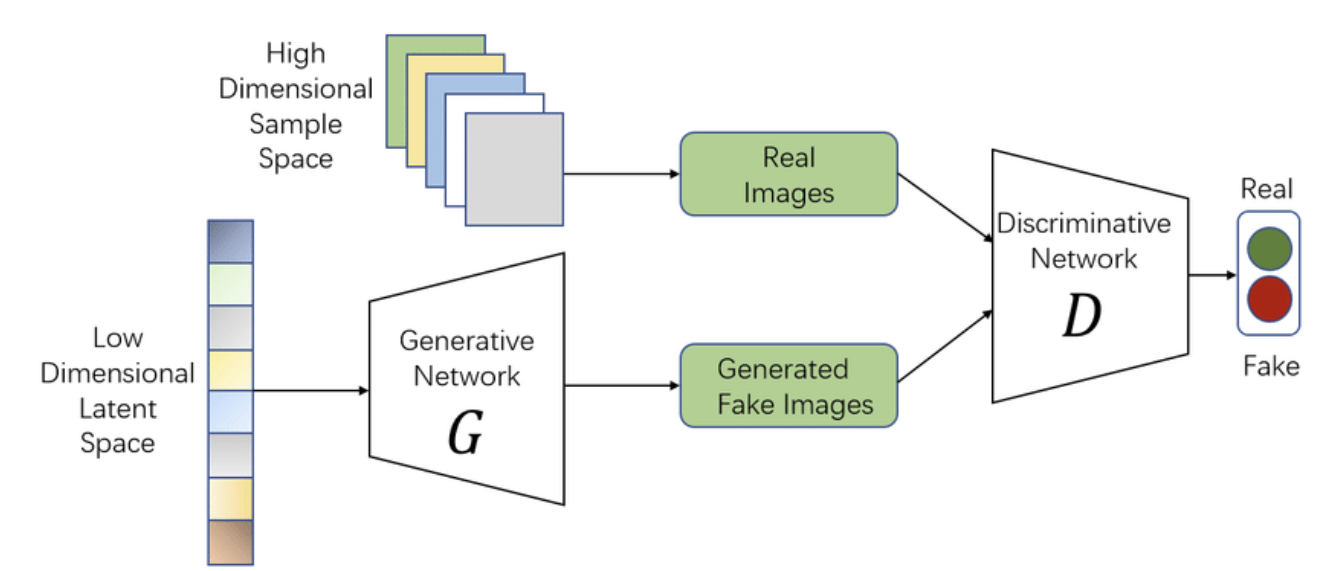
\includegraphics[width=\textwidth]{figChap1/gan-architect.png}\\
{\scriptsize Kiến trúc tổng quát GAN}
\end{column}
\end{columns}
\end{frame}

% --- Slide: Các biến thể GAN ---
\begin{frame}{Các giải pháp cải tiến GAN}
\begin{table}
\centering
\small
\begin{tabular}{p{3cm}p{4.5cm}p{5.5cm}}
\toprule
\textbf{Phương pháp} & \textbf{Ý tưởng} & \textbf{Vai trò trong DTGAN} \\
\midrule
\textbf{WGAN} & Wasserstein distance thay JS & Gradient có ý nghĩa hơn \\
\textbf{WGAN-GP} & Gradient Penalty & Ổn định huấn luyện \\
\textbf{SN-GAN} & Spectral Normalization & Dùng trong Discriminator DTGAN \\
\textbf{LSGAN} & Least Squares loss & Dùng trực tiếp trong DTGAN \\
\bottomrule
\end{tabular}
\end{table}

\vspace{0.3cm}
\begin{columns}[T]
\begin{column}{0.48\textwidth}
\textbf{Chỉ số đánh giá:}
\begin{itemize}
    \item \textbf{FID} (Fréchet Inception Distance): thấp hơn = tốt hơn
    \item \textbf{LPIPS}: đo khác biệt tri giác
\end{itemize}
\end{column}
\begin{column}{0.48\textwidth}
\centering
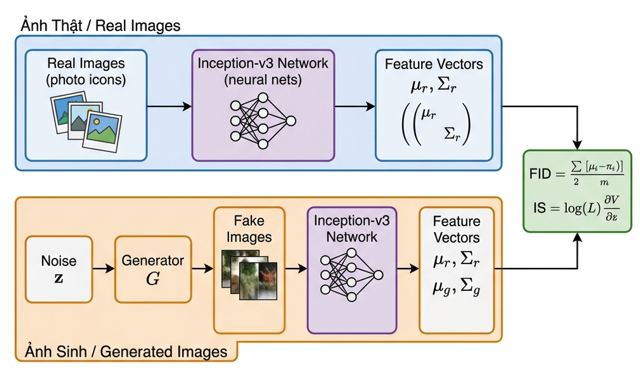
\includegraphics[width=0.85\textwidth]{figChap1/fid_is_pipeline.png}\\
{\scriptsize Quy trình tính FID/IS}
\end{column}
\end{columns}
\end{frame}

% --- Slide: So sánh các mô hình ---
\begin{frame}{So sánh các mô hình GAN cho bài toán Anime}
\begin{table}
\centering
\small
\begin{tabular}{lcccl}
\toprule
\textbf{Mô hình} & \textbf{FID $\downarrow$} & \textbf{Params (M)} & \textbf{Inference (ms)} & \textbf{Dữ liệu} \\
\midrule
CycleGAN & 86.7 & 28.3 & 42 & Không cặp \\
U-GAT-IT & 72.1 & 29.8 & 63 & Không cặp \\
AnimeGANv2 & 65.3 & 8.6 & 31 & Không cặp \\
\rowcolor{lightblue} \textbf{AnimeGANv3} & \textbf{58.4} & \textbf{1.02} & \textbf{12} & Không cặp \\
StyleGAN+Enc & 61.8 & 37.1 & 124 & Không cặp \\
\bottomrule
\end{tabular}
\end{table}

\vspace{0.2cm}
\begin{exampleblock}{Lý do chọn AnimeGANv3 (DTGAN)}
\textbf{FID thấp nhất} (58.4) $\cdot$ \textbf{Số tham số ít nhất} (1.02M) $\cdot$ \textbf{Tốc độ nhanh nhất} (12ms)
\end{exampleblock}
\end{frame}

% ============================================================================
% CHƯƠNG 2
% ============================================================================
\section{Kiến trúc DTGAN (AnimeGANv3)}

% --- Slide: Tổng quan DTGAN ---
\begin{frame}{Tổng quan kiến trúc DTGAN}
\centering
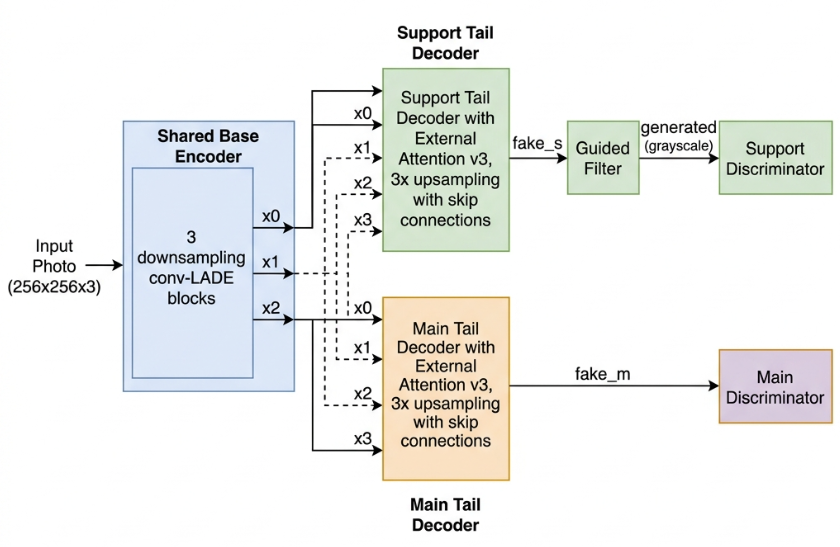
\includegraphics[width=0.88\textwidth]{figChap2/dtgan_architecture.png}\\
\vspace{0.2cm}
{\small \textbf{Ý tưởng trung tâm:} Tách quá trình học thành \textcolor{uetblue}{\textbf{hai nhiệm vụ song song}}}
\begin{columns}[T]
\begin{column}{0.32\textwidth}
\begin{block}{\centering Base Encoder}
\centering
\small
Shared weights\\
3$\times$ downsampling\\
$256^2 \to 32^2$
\end{block}
\end{column}
\begin{column}{0.32\textwidth}
\begin{block}{\centering Support Tail}
\centering
\small
Học đường nét, cấu trúc\\
Guided Filter\\
Grayscale D
\end{block}
\end{column}
\begin{column}{0.32\textwidth}
\begin{block}{\centering Main Tail}
\centering
\small
Tinh chỉnh màu, chi tiết\\
Pseudo GT\\
Full-color D
\end{block}
\end{column}
\end{columns}
\end{frame}

% --- Slide: LADE ---
\begin{frame}{Kỹ thuật chuẩn hóa LADE}
\begin{columns}[T]
\begin{column}{0.48\textwidth}
\textbf{LADE} (Linearly Adaptive Denormalization):

\vspace{0.2cm}
\textbf{Bước 1:} Chiếu tuyến tính
$$t_x = \text{Conv}_{1\times1}(x)$$

\textbf{Bước 2:} Tính thống kê thích ứng
$$(\mu_t, \sigma_t^2) = \text{moments}(t_x)$$

\textbf{Bước 3:} Normalize + Denormalize
$$\text{LADE}(x) = \frac{x - \mu_x}{\sqrt{\sigma_x^2 + \varepsilon}} \cdot \sqrt{\sigma_t^2 + \varepsilon} + \mu_t$$

\vspace{0.1cm}
{\small $\Rightarrow$ \textbf{Tự động học} tham số từ chính feature map, không cần ảnh style riêng}
\end{column}
\begin{column}{0.48\textwidth}
\centering
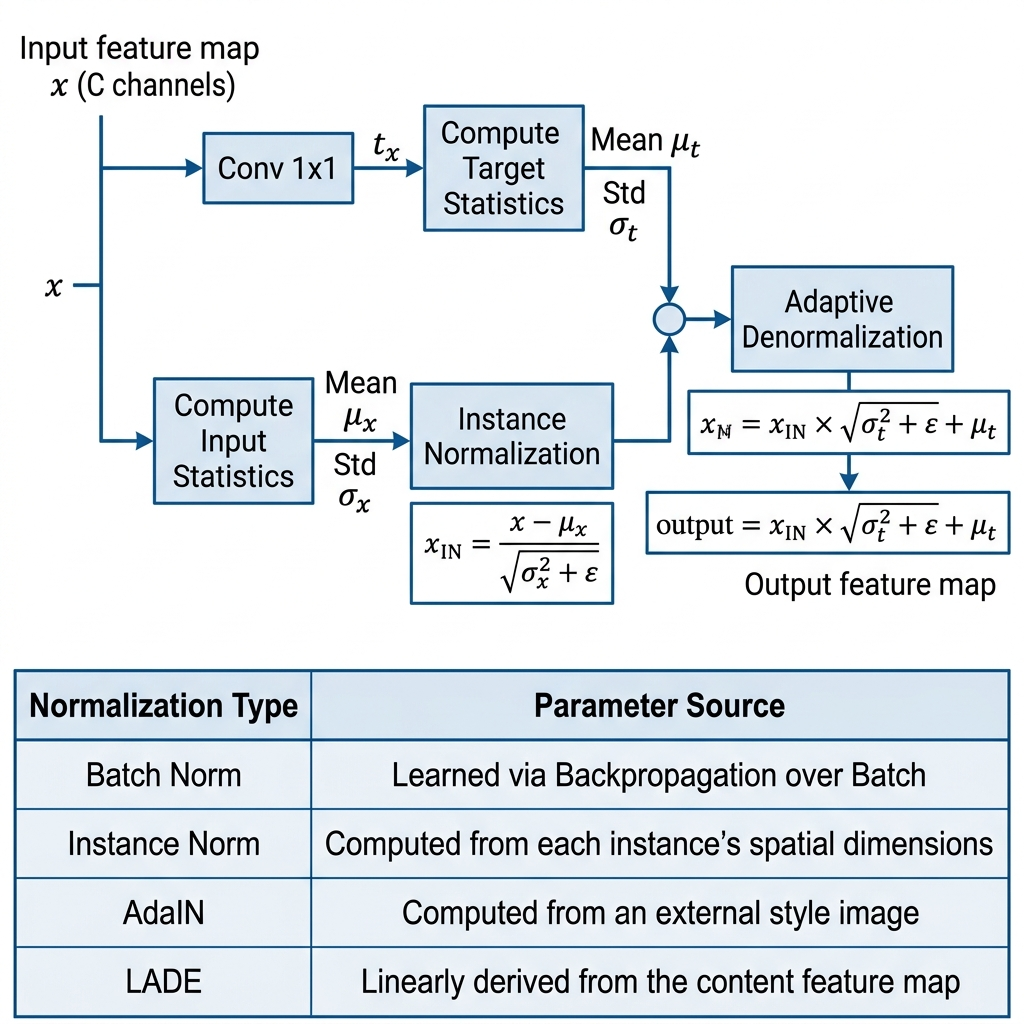
\includegraphics[width=\textwidth]{figChap2/lade_normalization.png}\\
{\scriptsize Cơ chế hoạt động LADE}

\vspace{0.3cm}
\small
\begin{tabular}{ll}
\toprule
\textbf{Kỹ thuật} & \textbf{Nguồn tham số} \\
\midrule
Batch Norm & Thống kê batch \\
Instance Norm & $\gamma, \beta$ cố định \\
AdaIN & Ảnh style riêng \\
\textcolor{uetblue}{\textbf{LADE}} & \textcolor{uetblue}{\textbf{Conv $1\times1$ trên $x$}} \\
\bottomrule
\end{tabular}
\end{column}
\end{columns}
\end{frame}

% --- Slide: External Attention ---
\begin{frame}{External Attention v3 \& Discriminator}
\begin{columns}[T]
\begin{column}{0.48\textwidth}
\textbf{External Attention v3:}
\begin{itemize}
    \item Thay Self-Attention ($O(N^2)$) bằng learnable memory banks $M_k, M_v$
    \item Độ phức tạp: $O(N \cdot k)$, $k \ll N$
    \item Double normalization tránh attention head chiếm ưu thế
\end{itemize}

\centering
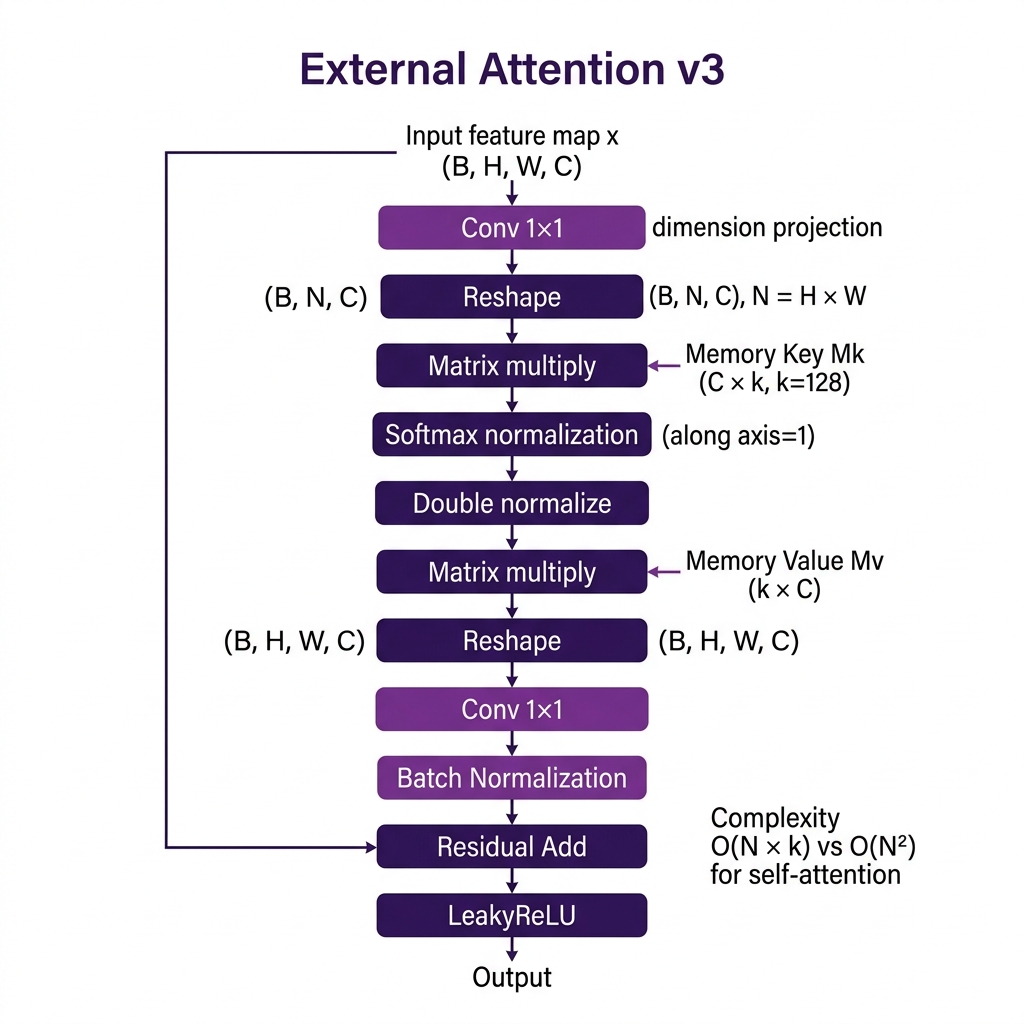
\includegraphics[width=0.9\textwidth]{figChap2/external_attention.png}\\
{\scriptsize External Attention v3 tại bottleneck $32\times32$}
\end{column}
\begin{column}{0.48\textwidth}
\textbf{Hai Discriminator PatchGAN:}

\vspace{0.2cm}
\begin{alertblock}{Support D (Grayscale)}
\small
Phân biệt ảnh anime đen trắng vs. $\hat{y}$\\
$\to$ Tập trung đường nét, tương phản
\end{alertblock}

\begin{exampleblock}{Main D (Full-color RGB)}
\small
Phân biệt anime sạch (NL-Means + L0) vs. $\hat{y}_m$\\
$\to$ Kiểm soát cel-shading, màu sắc mịn
\end{exampleblock}

\vspace{0.1cm}
{\small Cả hai sử dụng \textbf{LADE\_D} = LADE + Spectral Norm}
\end{column}
\end{columns}
\end{frame}

% --- Slide: Hệ thống Loss ---
\begin{frame}{Hệ thống Hàm Mất mát Đa thành phần}
\centering
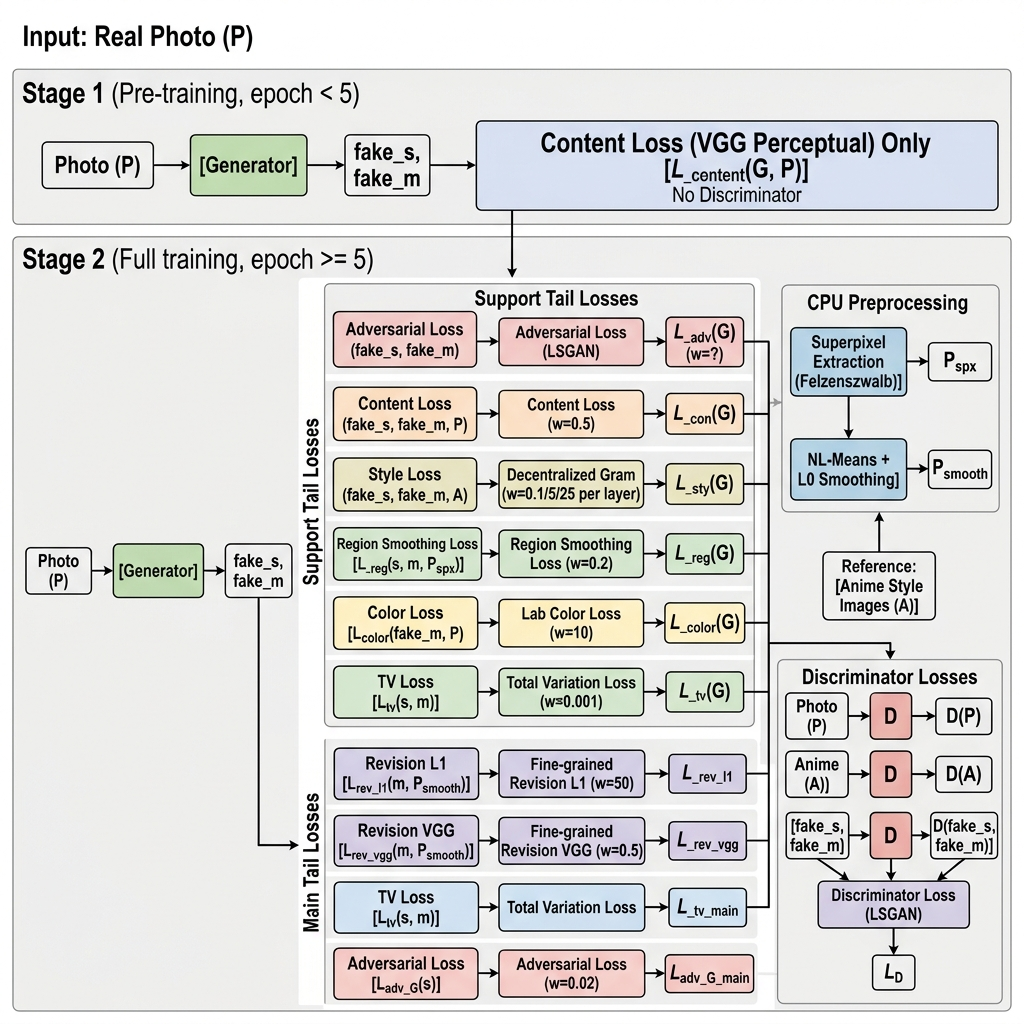
\includegraphics[width=0.75\textwidth]{figChap2/loss_functions_diagram.png}

\vspace{0.2cm}
\begin{columns}[T]
\begin{column}{0.48\textwidth}
\textbf{Support Tail:}
\begin{itemize}
    \small
    \item Content Loss (VGG19 conv4\_4)
    \item Style Loss (Decentralized Gram)
    \item Region Smoothing (Superpixel)
    \item Lab Color Loss
    \item TV Loss + LSGAN Adv Loss
\end{itemize}
\end{column}
\begin{column}{0.48\textwidth}
\textbf{Main Tail:}
\begin{itemize}
    \small
    \item Fine-grained Revision Loss
    \item Pseudo GT: NL-Means + L0 Smooth
    \item TV Loss + LSGAN Adv Loss (nhẹ)
\end{itemize}

\vspace{0.2cm}
\textbf{Huấn luyện 2 giai đoạn:}
\begin{itemize}
    \small
    \item GĐ1: Pre-training (5 epoch, chỉ Content Loss)
    \item GĐ2: Adversarial đầy đủ (69 epoch)
\end{itemize}
\end{column}
\end{columns}
\end{frame}

% ============================================================================
% CHƯƠNG 3
% ============================================================================
\section{Pipeline tích hợp phát hiện khuôn mặt}

% --- Slide: Pipeline tổng quan ---
\begin{frame}{Pipeline Tích hợp Face Extraction — Đóng góp chính}
\centering
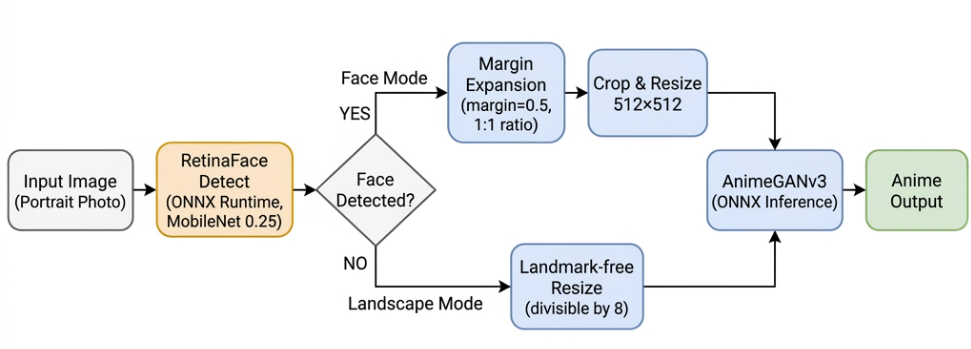
\includegraphics[width=0.82\textwidth]{figChap3/face_extraction_pipeline.png}

\vspace{0.3cm}
\begin{columns}[T]
\begin{column}{0.30\textwidth}
\begin{block}{\centering Face Mode}
\small
\centering
RetinaFace $\to$ Crop\\
$512\times512$ $\to$ ONNX\\
\textbf{Chất lượng mặt cao}
\end{block}
\end{column}
\begin{column}{0.30\textwidth}
\begin{block}{\centering Landscape Mode}
\small
\centering
Resize to\_8s\\
Giữ toàn cảnh\\
\textbf{Bảo toàn bố cục}
\end{block}
\end{column}
\begin{column}{0.35\textwidth}
\begin{block}{\centering Hybrid Mode}
\small
\centering
Nền: Landscape\\
Mặt: Face Mode riêng\\
\textbf{Feathered blending}
\end{block}
\end{column}
\end{columns}
\end{frame}

% --- Slide: RetinaFace ---
\begin{frame}{Phát hiện khuôn mặt — RetinaFace MobileNet 0.25}
\begin{columns}[T]
\begin{column}{0.50\textwidth}
\centering
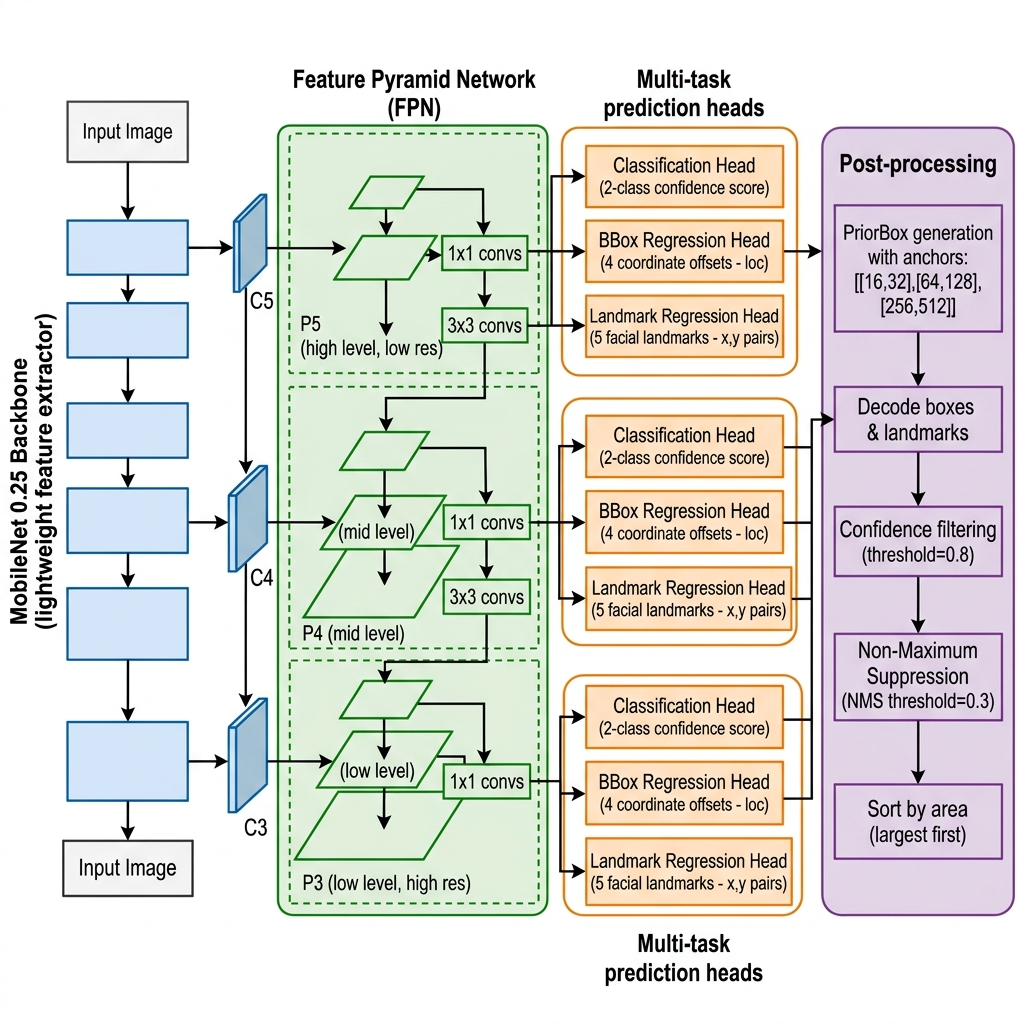
\includegraphics[width=\textwidth]{figChap3/retinaface_architecture.png}\\
{\scriptsize Kiến trúc RetinaFace với FPN đa tỉ lệ}
\end{column}
\begin{column}{0.46\textwidth}
\textbf{Kiến trúc 3 thành phần:}
\begin{enumerate}
    \small
    \item \textbf{Backbone MobileNet 0.25}: Depthwise Separable Conv, giảm 8-9$\times$ tính toán
    \item \textbf{FPN đa tỉ lệ}: $P_3, P_4, P_5$ phát hiện mọi kích thước mặt
    \item \textbf{Multi-task Heads}: Classification + BBox + 5 Landmarks
\end{enumerate}

\vspace{0.2cm}
\textbf{Hậu xử lý:}
\begin{itemize}
    \small
    \item Confidence $> 0.8$
    \item NMS (IoU $> 0.3$)
    \item Sắp xếp theo diện tích
\end{itemize}
\end{column}
\end{columns}
\end{frame}

% --- Slide: Margin Expansion ---
\begin{frame}{Thuật toán Margin Expansion}
\begin{columns}[T]
\begin{column}{0.52\textwidth}
\centering
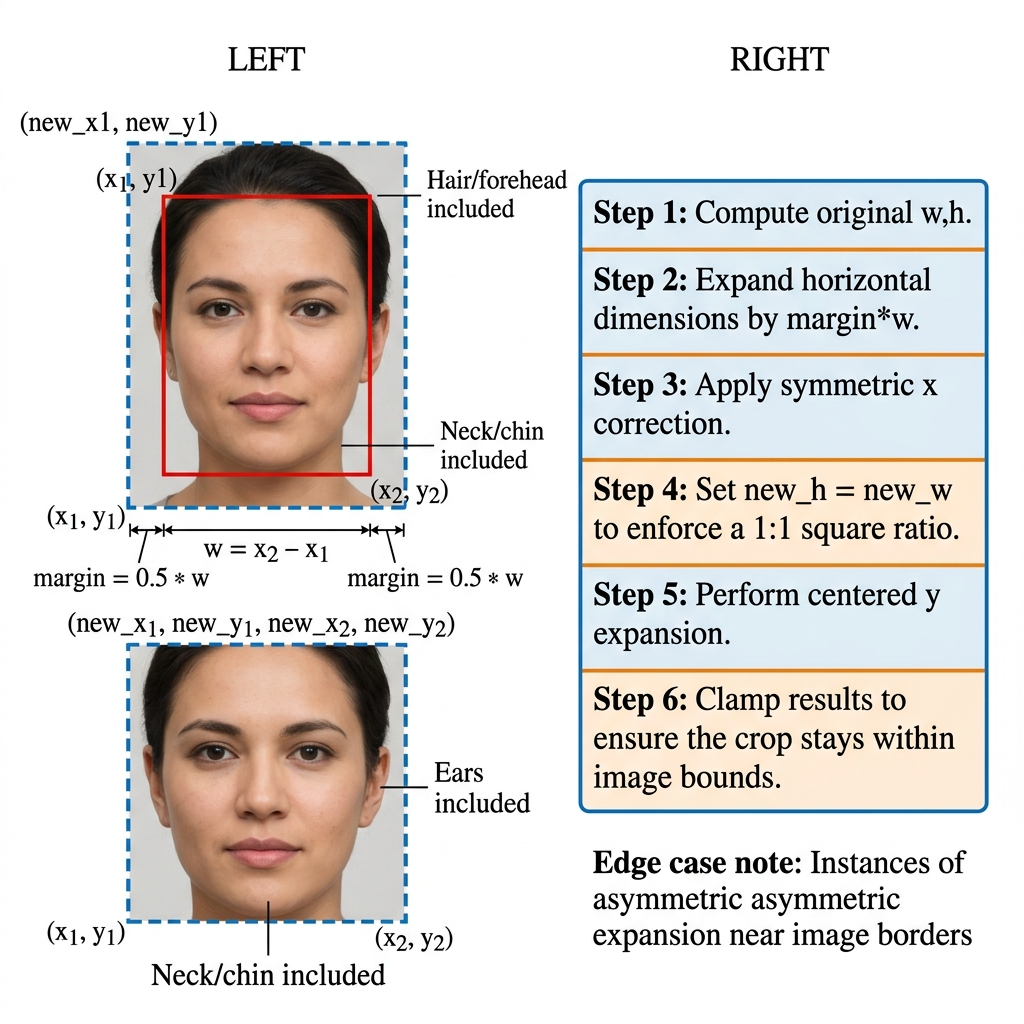
\includegraphics[width=0.85\textwidth]{figChap3/margin_expansion.png}\\
{\scriptsize Mở rộng 50\% mỗi bên, đảm bảo tỉ lệ 1:1}
\end{column}
\begin{column}{0.45\textwidth}
\textbf{6 bước thuật toán} ($m = 0.5$):
\begin{enumerate}
    \small
    \item Tính kích thước hộp gốc: $w, h$
    \item Mở rộng ngang: $x_1' = x_1 - m \cdot w$
    \item Đảm bảo đối xứng: $x_d = \min(\Delta_L, \Delta_R)$
    \item Chiều cao mới: $h' = w'$ (tỉ lệ 1:1)
    \item Điều chỉnh dọc (phân nhánh)
    \item Clamp về biên ảnh
\end{enumerate}

\vspace{0.1cm}
\textbf{Bao phủ:} Tóc, tai, cổ, phần trên vai\\
\textbf{Edge cases:} Mặt gần biên, góc ảnh, mặt rất lớn
\end{column}
\end{columns}
\end{frame}

% --- Slide: Hybrid Mode ---
\begin{frame}{Hybrid Mode — Feathered Blending}
\begin{columns}[T]
\begin{column}{0.52\textwidth}
\centering
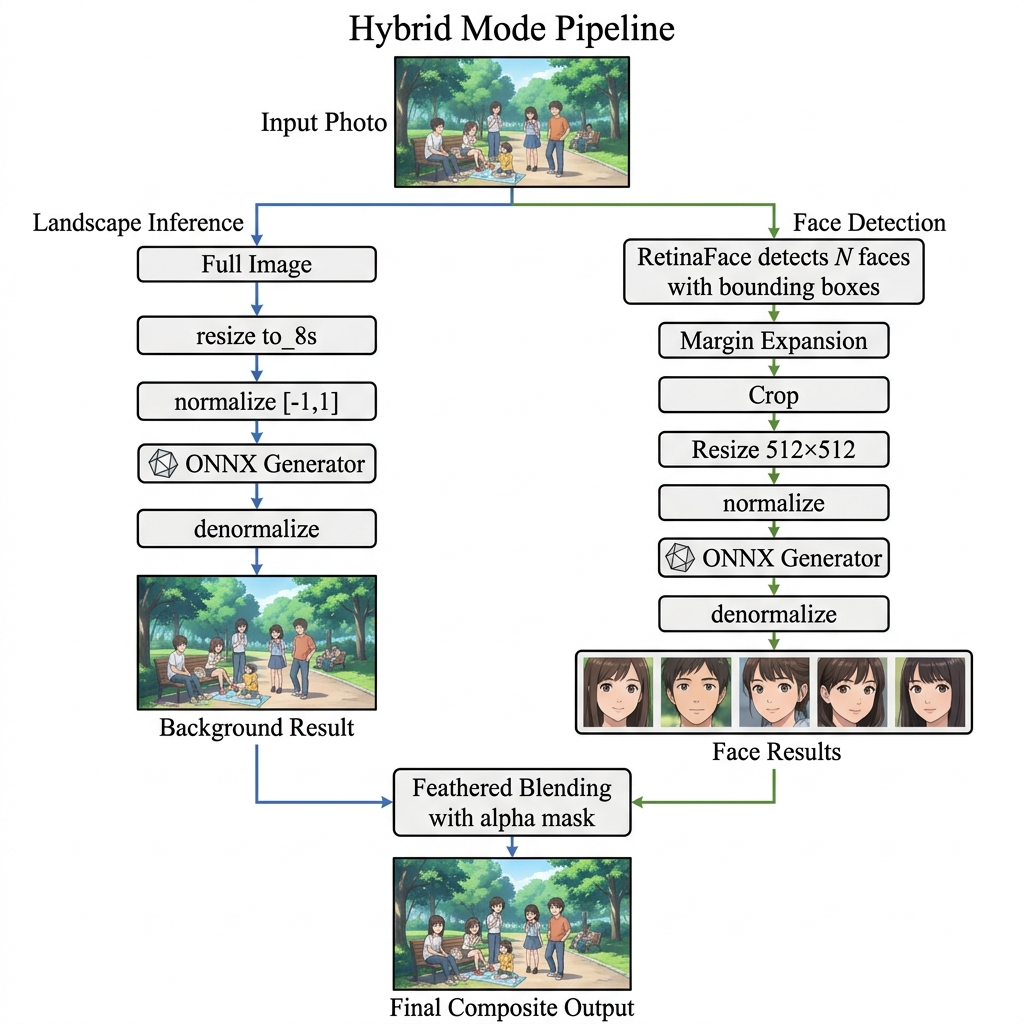
\includegraphics[width=\textwidth]{figChap3/hybrid_mode_pipeline.png}\\
{\scriptsize Pipeline Hybrid Mode}

\vspace{0.2cm}
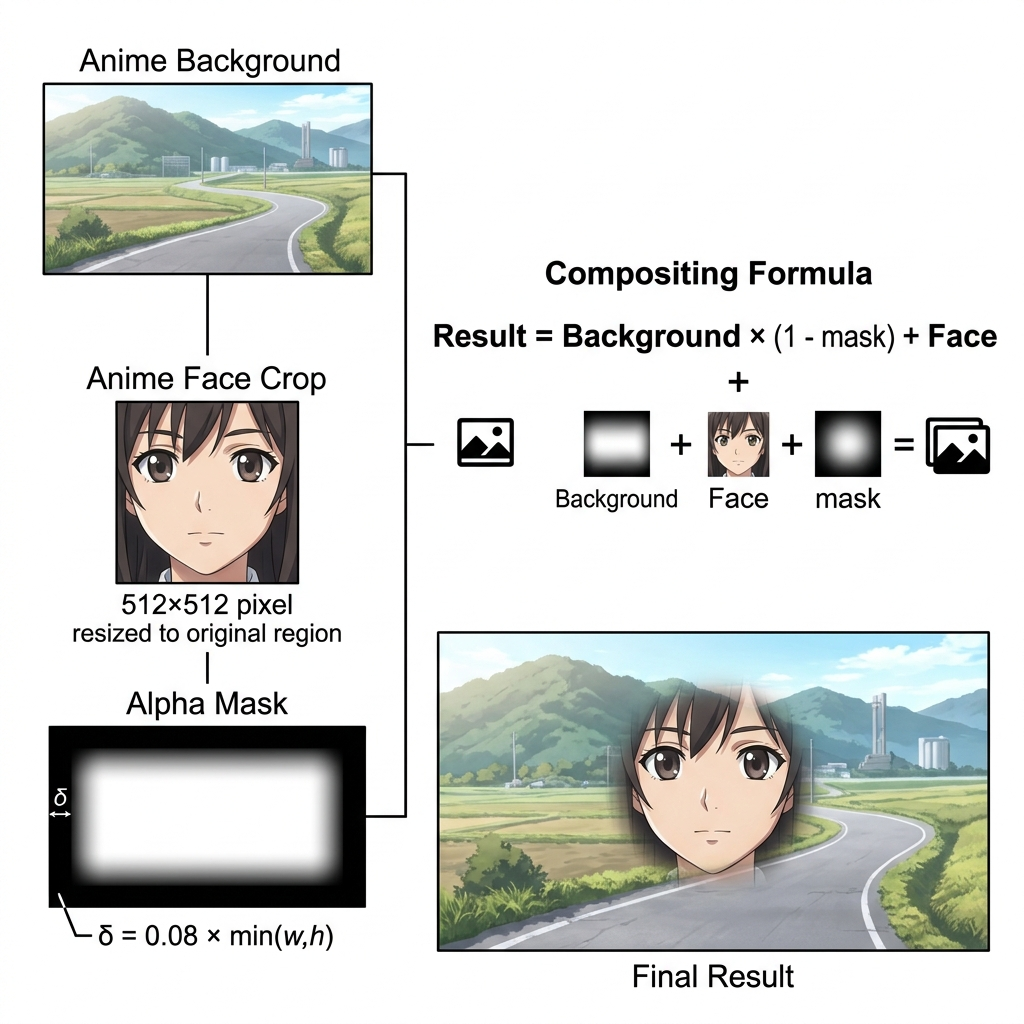
\includegraphics[width=\textwidth]{figChap3/feathered_blending.png}\\
{\scriptsize Feathered Blending: alpha mask Gaussian}
\end{column}
\begin{column}{0.44\textwidth}
\textbf{4 giai đoạn:}
\begin{enumerate}
    \small
    \item Phát hiện tất cả khuôn mặt
    \item Suy luận nền (Landscape)
    \item Suy luận từng mặt ($512^2$)
    \item Ghép bằng alpha compositing
\end{enumerate}

\vspace{0.2cm}
\textbf{Alpha compositing:}
$$I_{\text{out}} = \frac{\hat{M}}{255} \cdot I_{\text{face}} + (1-\frac{\hat{M}}{255}) \cdot I_{\text{bg}}$$

\vspace{0.1cm}
{\small $\delta = 8\%$ kích thước cạnh nhỏ hơn}

\vspace{0.2cm}
\textbf{Graceful degradation:}\\
{\small Không phát hiện mặt $\to$ tự động Landscape}
\end{column}
\end{columns}
\end{frame}

% ============================================================================
% CHƯƠNG 4
% ============================================================================
\section{Thực nghiệm và Đánh giá}

% --- Slide: Môi trường ---
\begin{frame}{Môi trường Thực nghiệm}
\begin{columns}[T]
\begin{column}{0.48\textwidth}
\begin{block}{Phần cứng (vast.ai)}
\small
\begin{tabular}{ll}
\textbf{GPU} & NVIDIA RTX A5000 (24GB) \\
\textbf{CPU} & Intel i9-10900X (10C/20T) \\
\textbf{RAM} & 64 GB \\
\textbf{SSD} & 2TB ($\sim$3090 MB/s) \\
\end{tabular}
\end{block}
\end{column}
\begin{column}{0.48\textwidth}
\begin{block}{Phần mềm}
\small
\begin{tabular}{ll}
\textbf{Framework} & TensorFlow 1.12 \\
\textbf{Runtime} & ONNX Runtime 1.13 \\
\textbf{Backend} & FastAPI \\
\textbf{Frontend} & React 19 \\
\end{tabular}
\end{block}
\end{column}
\end{columns}

\vspace{0.3cm}
\begin{block}{Bộ dữ liệu}
\begin{itemize}
    \small
    \item \textbf{Ảnh thực:} Ảnh chân dung đa dạng (giới tính, tuổi, sắc tộc, ánh sáng). Tiền xử lý: Felzenszwalb superpixel ($\sigma$=5, k=0.8, min\_size=50)
    \item \textbf{Ảnh anime:} Frame phim Hayao Miyazaki (\textit{Spirited Away}, \textit{Totoro}), Makoto Shinkai (\textit{Your Name}). Tiền xử lý: Edge Smoothing
\end{itemize}
\end{block}
\end{frame}

% --- Slide: Kết quả huấn luyện ---
\begin{frame}{Kết quả Huấn luyện — Đường cong Hội tụ}
\begin{columns}[T]
\begin{column}{0.48\textwidth}
\centering
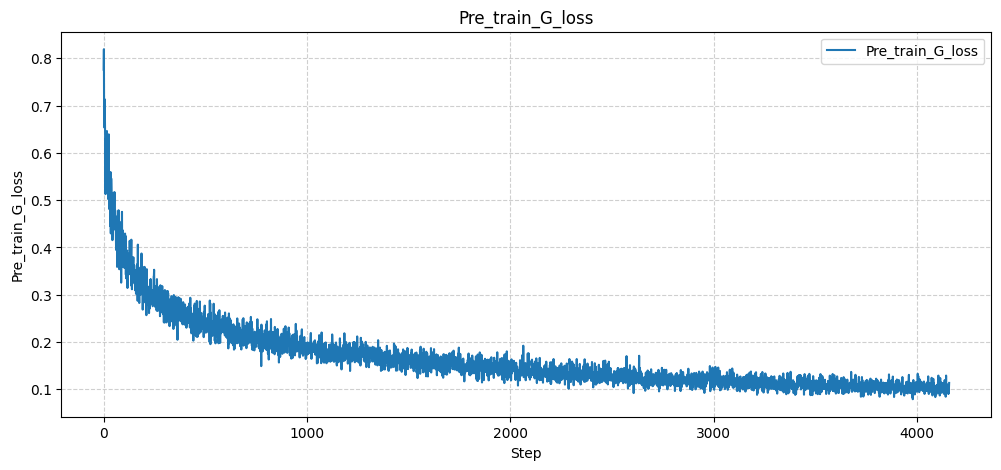
\includegraphics[width=\textwidth]{figChap3/preTrainGLoss.png}\\
{\scriptsize Pre-train G\_loss: $1.74 \to 0.25$ (5 epoch)}
\end{column}
\begin{column}{0.48\textwidth}
\centering
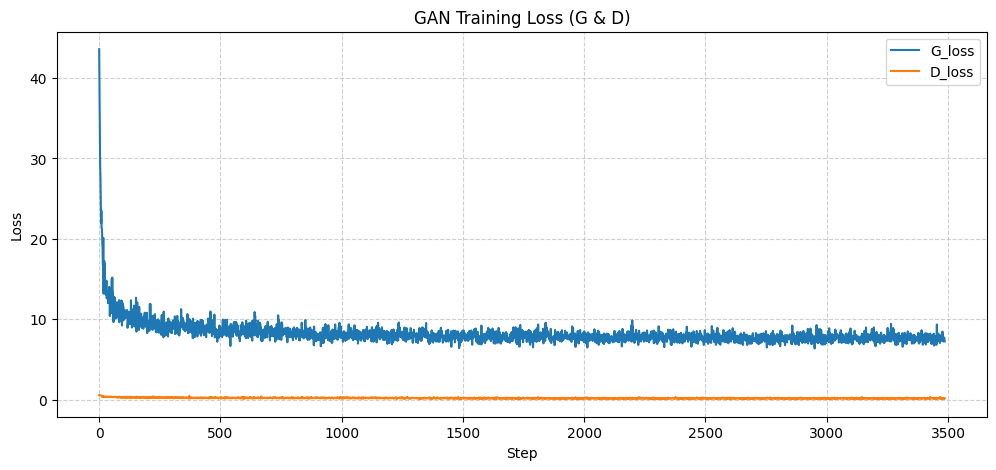
\includegraphics[width=\textwidth]{figChap3/Dloss_Gloss.png}\\
{\scriptsize G\_loss (xanh) $\approx 6.5$; D\_loss (cam) $\approx 0.11$}
\end{column}
\end{columns}

\vspace{0.2cm}
\begin{exampleblock}{Nhận xét}
\small
\begin{itemize}
    \item Pre-training hội tụ mượt mà, đặt nền tảng ổn định cho adversarial
    \item D\_loss nhỏ và ổn định $\Rightarrow$ không xảy ra mode collapse
    \item G\_loss dao động $[5.6, 9.0]$ là bình thường — phản ánh ``cạnh tranh'' G-D liên tục
\end{itemize}
\end{exampleblock}
\end{frame}

% --- Slide: Các thành phần Loss ---
\begin{frame}{Các thành phần Loss phụ}
\centering
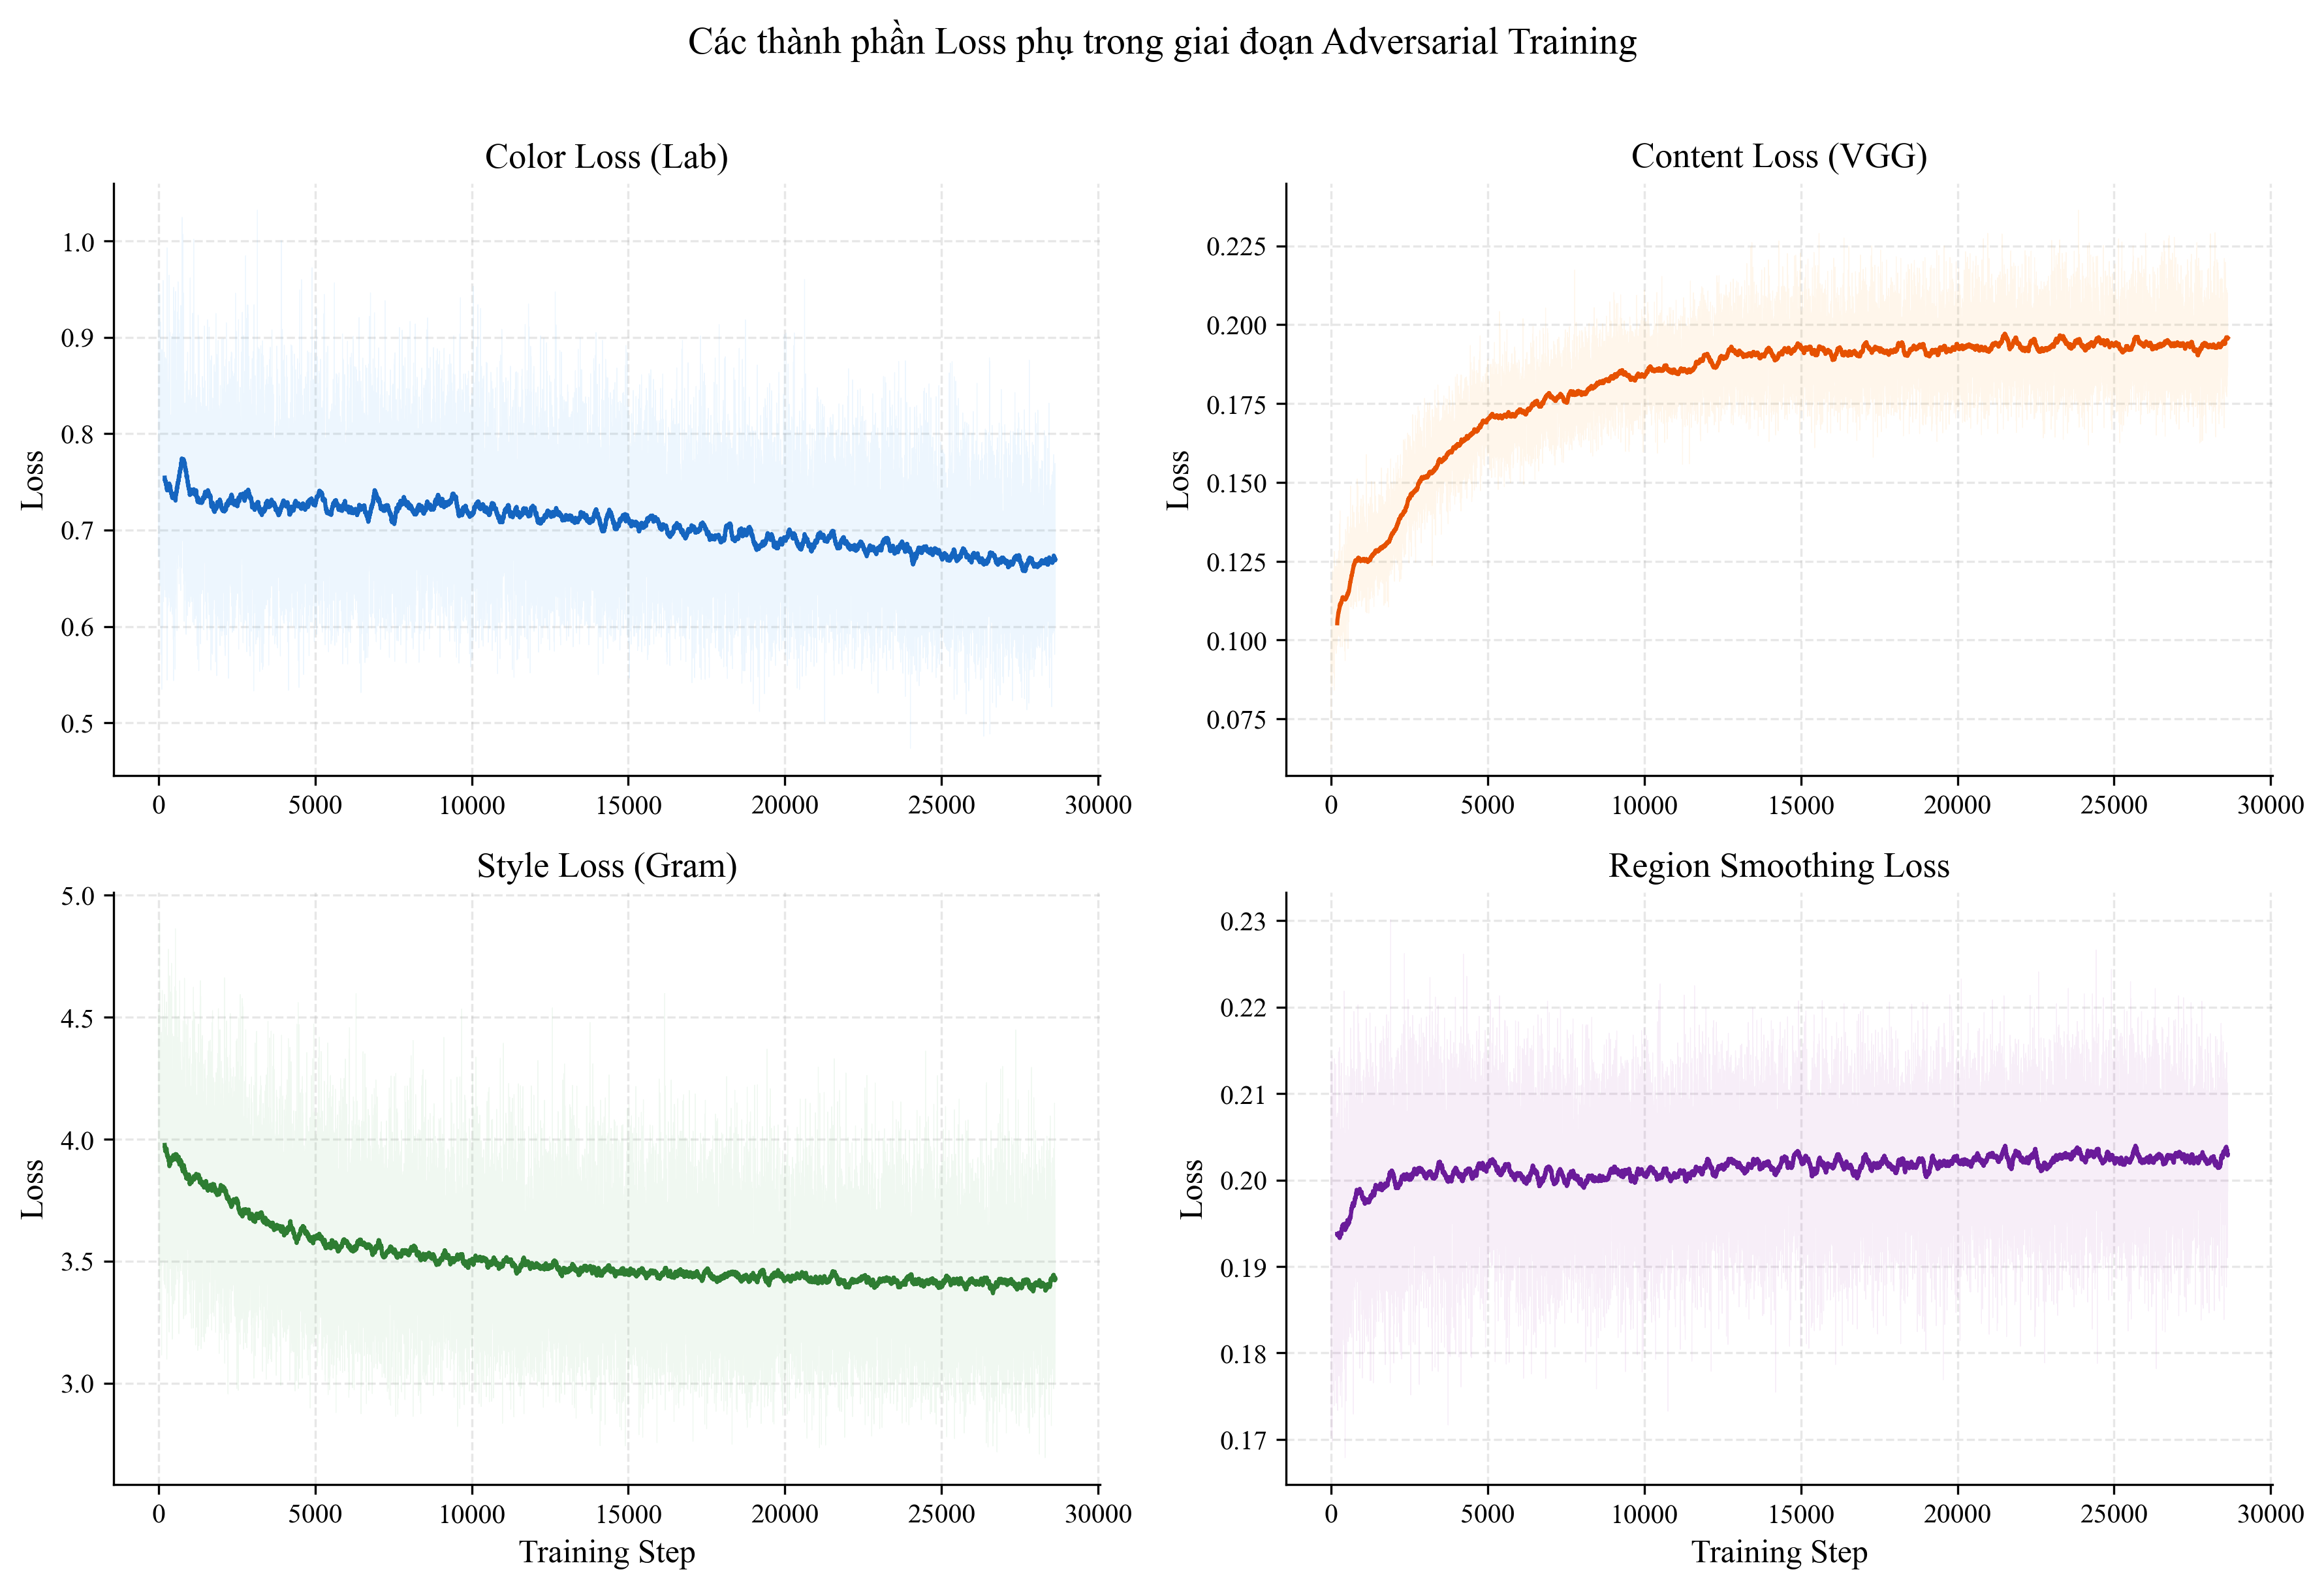
\includegraphics[width=0.75\textwidth]{figChap3/component_losses.png}

\vspace{0.2cm}
\begin{columns}
\begin{column}{0.24\textwidth}
\centering
\textbf{Content}\\
$\approx 0.19 \pm 0.01$\\
{\scriptsize Bảo toàn nội dung tốt}
\end{column}
\begin{column}{0.24\textwidth}
\centering
\textbf{Color}\\
$\approx 0.67 \pm 0.05$\\
{\scriptsize Màu sắc nhất quán}
\end{column}
\begin{column}{0.24\textwidth}
\centering
\textbf{Style}\\
$\approx 3.42 \pm 0.24$\\
{\scriptsize Học phong cách anime}
\end{column}
\begin{column}{0.24\textwidth}
\centering
\textbf{Region Smooth}\\
$\approx 0.20 \pm 0.01$\\
{\scriptsize Vùng mịn ổn định}
\end{column}
\end{columns}
\end{frame}

% --- Slide: Đánh giá định lượng ---
\begin{frame}{Đánh giá Định lượng — So sánh với Baseline}
\begin{table}
\centering
\small
\begin{tabular}{lcccc}
\toprule
\textbf{Phương pháp} & \textbf{FID $\downarrow$} & \textbf{LPIPS $\downarrow$} & \textbf{FPS (GPU)} & \textbf{Model (MB)} \\
\midrule
CycleGAN & 98.4 & 0.512 & 18 & 44 \\
CartoonGAN & 84.7 & 0.487 & 24 & 38 \\
AnimeGANv2 & 72.3 & 0.421 & 31 & 8.6 \\
\rowcolor{lightblue} \textbf{AnimeGANv3 (Face)} & \textbf{58.6} & \textbf{0.384} & \textbf{42} & \textbf{9.1} \\
AnimeGANv3 (Landscape) & 64.2 & 0.409 & 38 & 9.1 \\
AnimeGANv3 (Hybrid) & 60.1 & 0.391 & -- & 9.1 \\
\bottomrule
\end{tabular}
\end{table}

\vspace{0.2cm}
\begin{columns}
\begin{column}{0.48\textwidth}
\begin{exampleblock}{\centering Điểm nổi bật}
\centering
\small
\textbf{Face Mode: FID 58.6} (tốt nhất)\\
Cải thiện \textbf{$\sim$8.7\%} so với Landscape
\end{exampleblock}
\end{column}
\begin{column}{0.48\textwidth}
\begin{block}{\centering Hiệu năng}
\centering
\small
Model ONNX chỉ \textbf{9.1 MB}\\
\textbf{42 FPS} @ $256\times256$ GPU
\end{block}
\end{column}
\end{columns}
\end{frame}

% --- Slide: Đánh giá định tính ---
\begin{frame}{Đánh giá Định tính — So sánh ba Chế độ}
\begin{columns}
\begin{column}{0.24\textwidth}
\centering
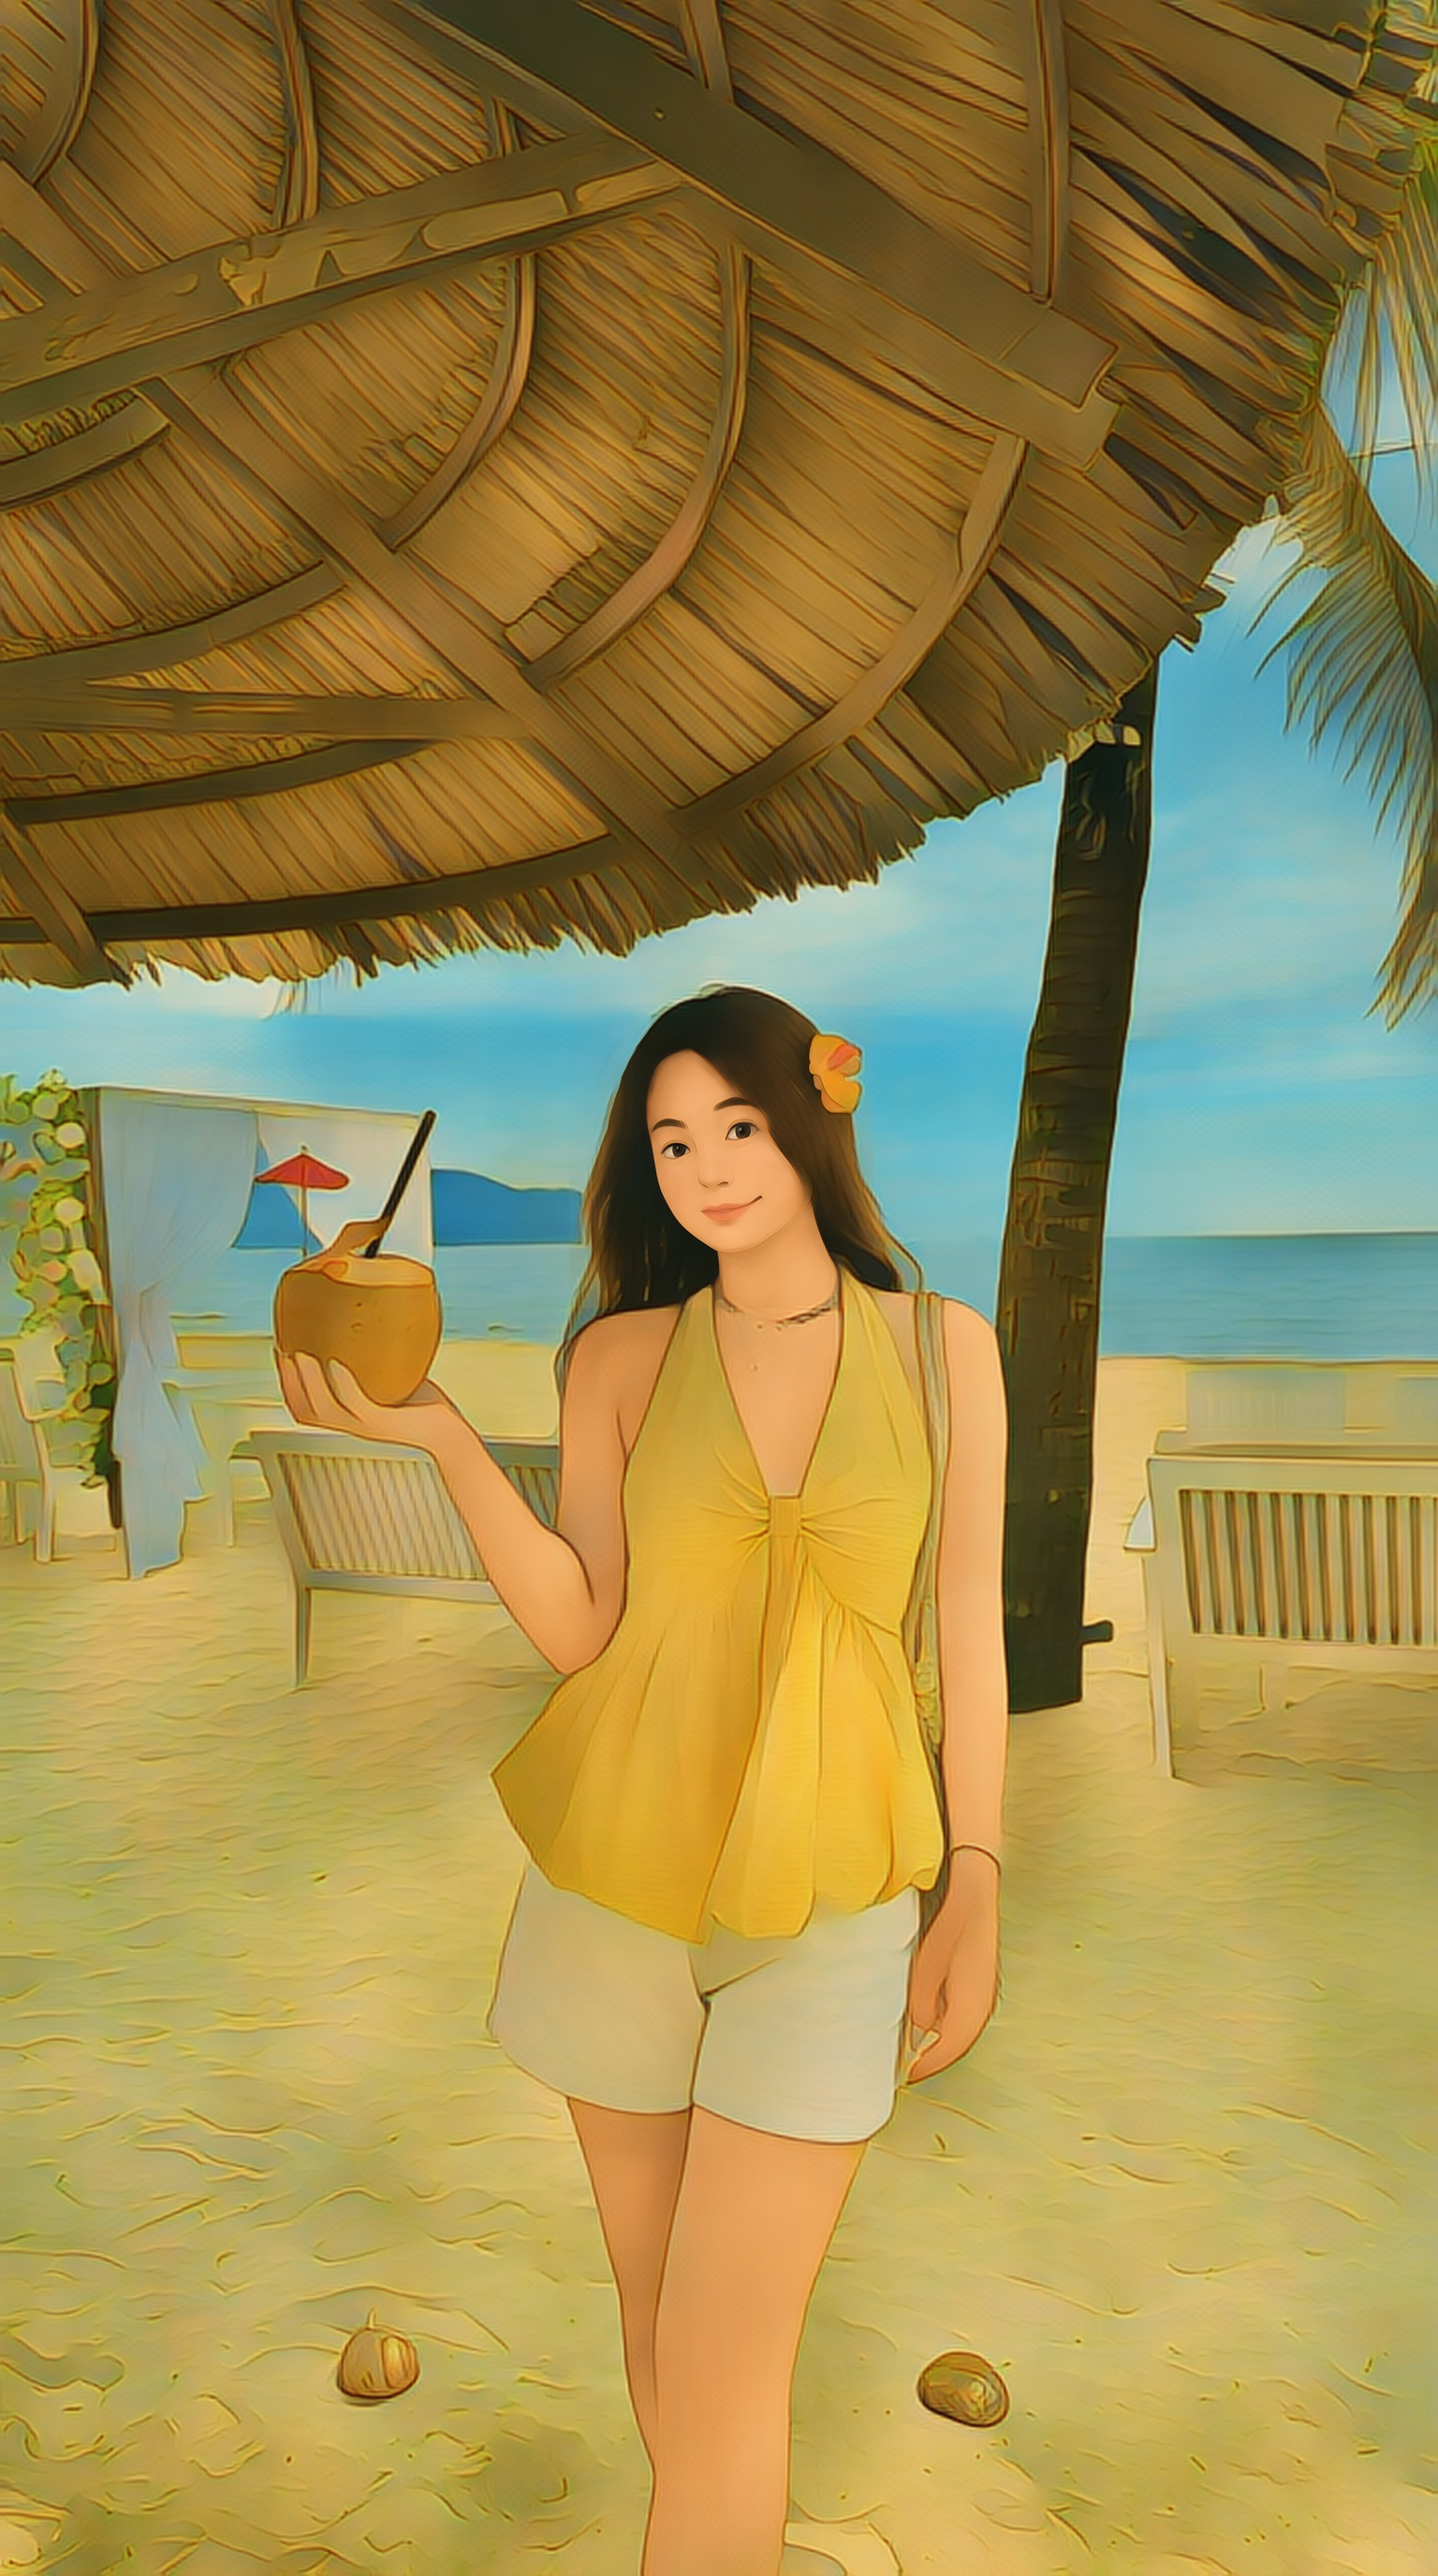
\includegraphics[width=\textwidth]{figChap3/style_results/e1.jpg}\\
{\scriptsize (a) Hybrid Mode}
\end{column}
\begin{column}{0.24\textwidth}
\centering
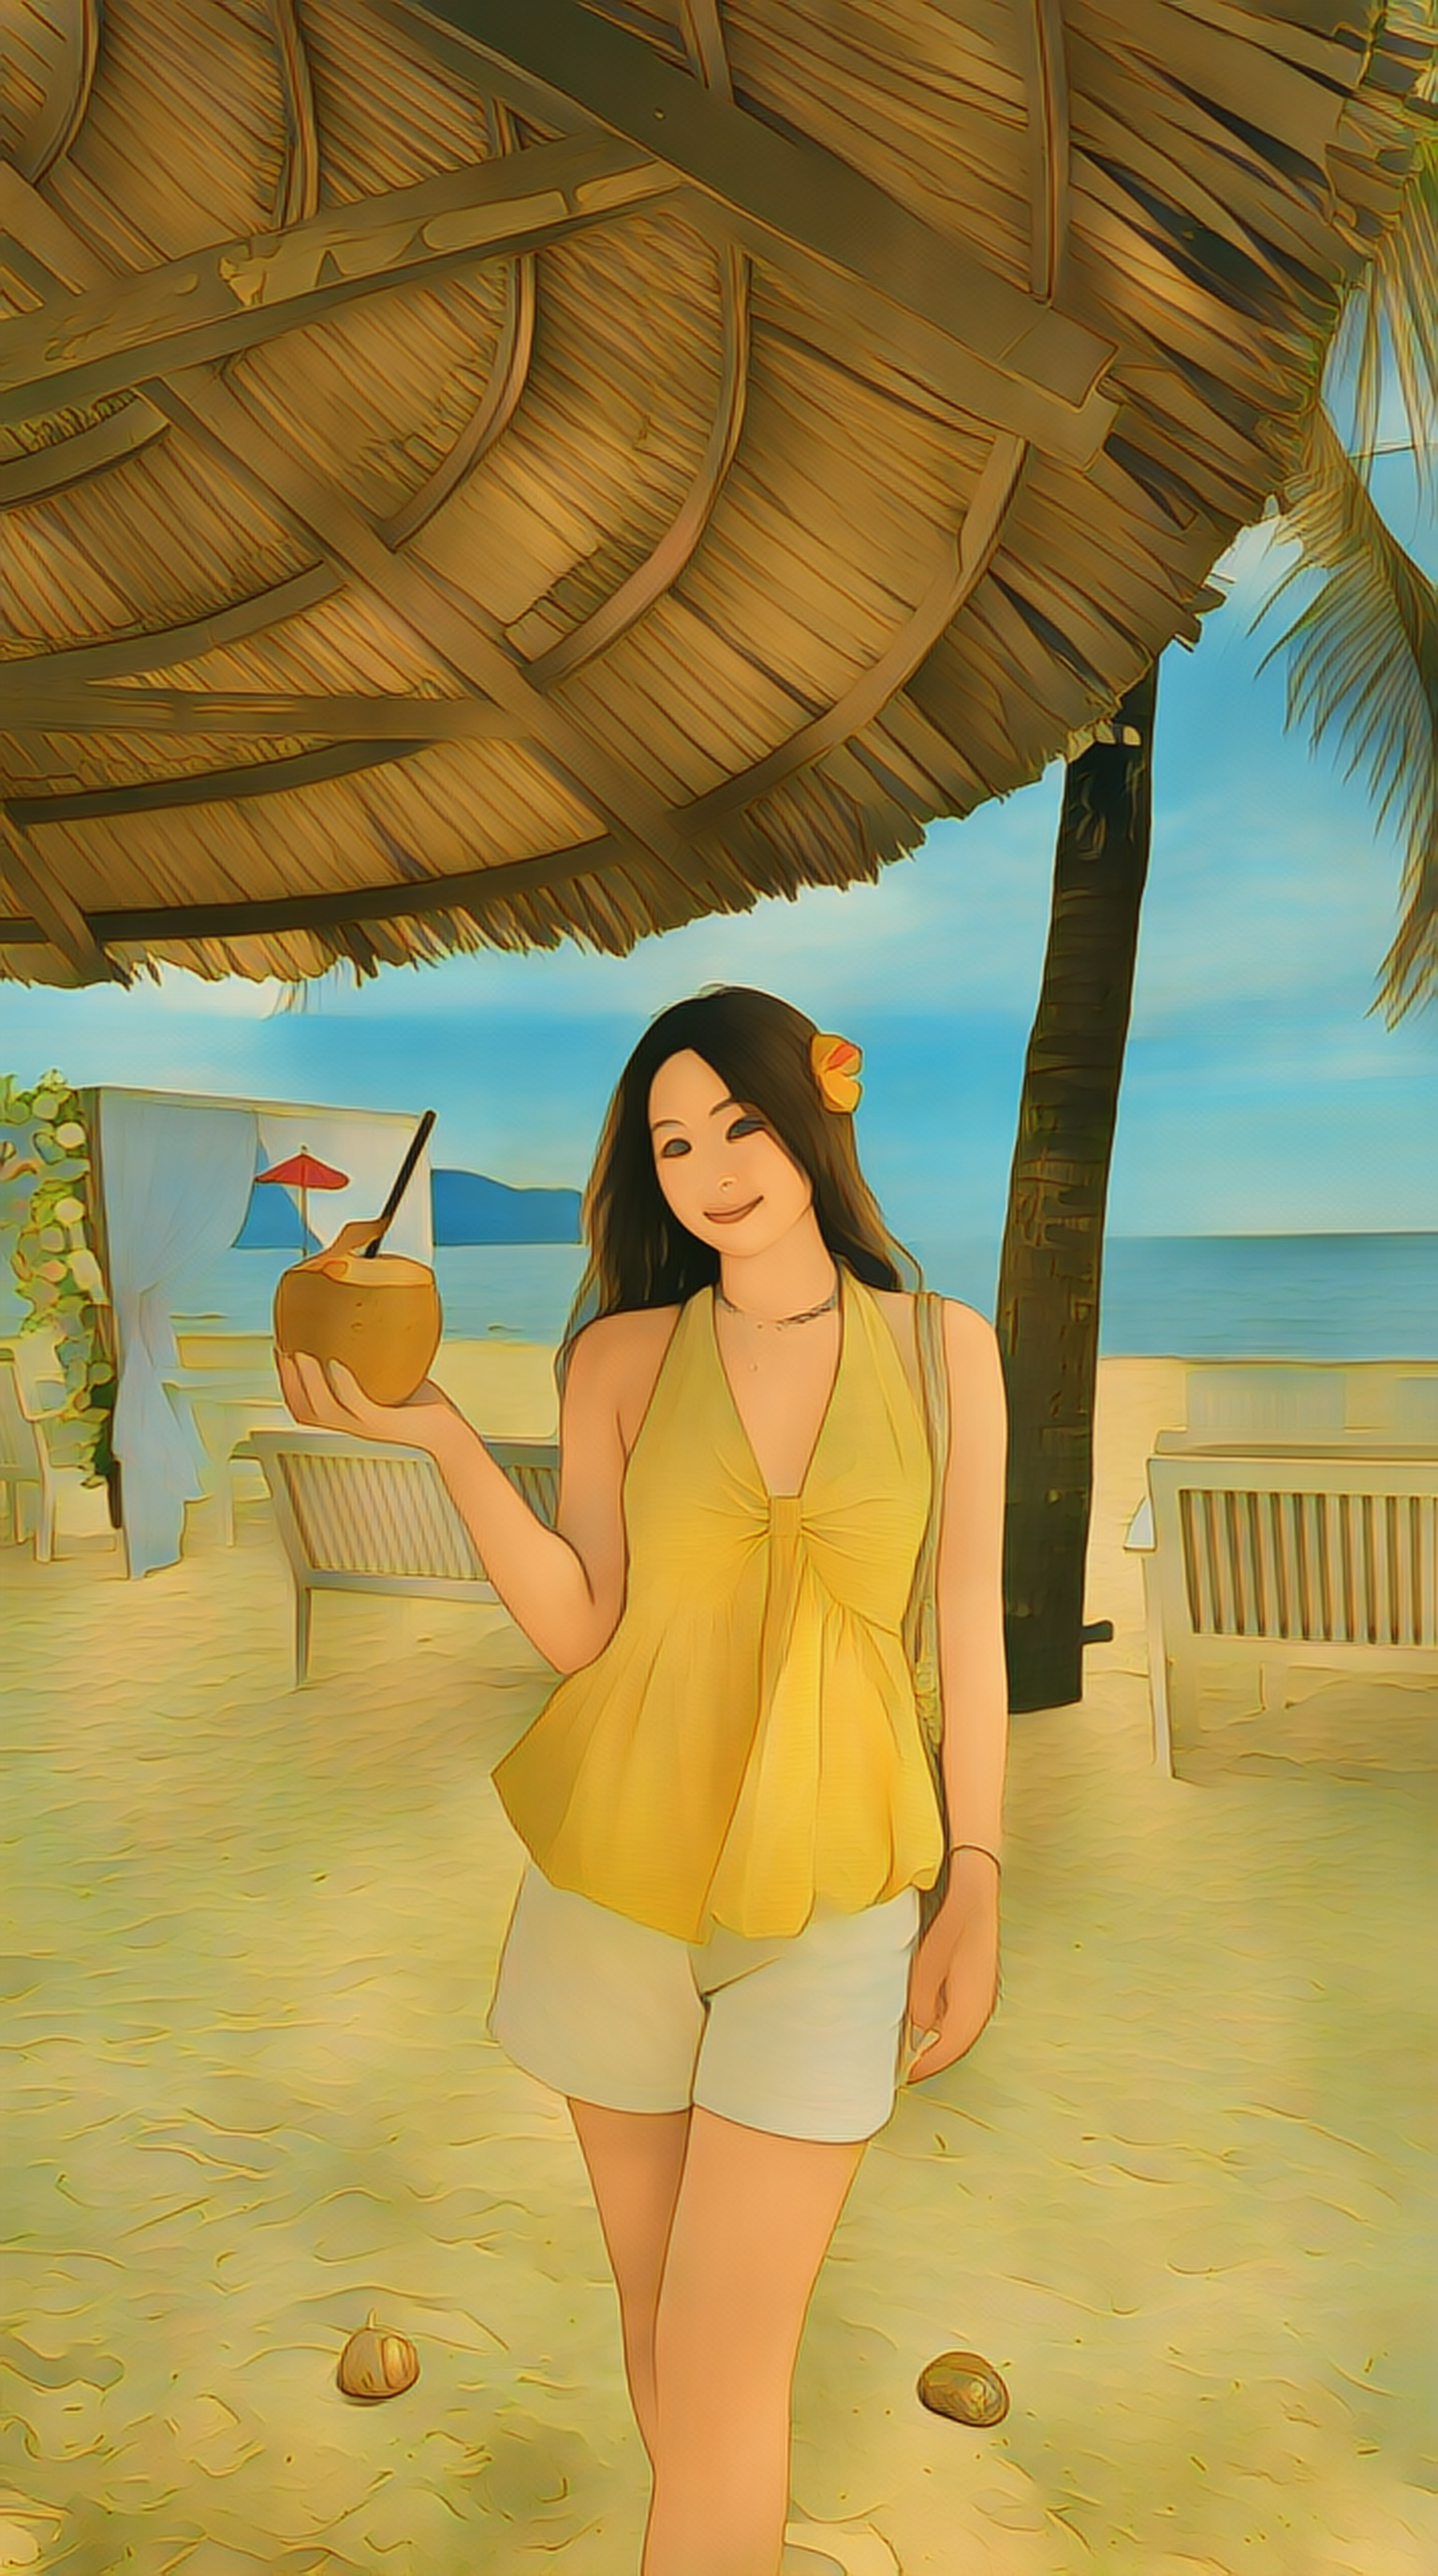
\includegraphics[width=\textwidth]{figChap3/style_results/b1.jpg}\\
{\scriptsize (b) Landscape Mode}
\end{column}
\begin{column}{0.24\textwidth}
\centering

\includegraphics[width=\textwidth]{figChap3/style_results/c1.png}\\
{\scriptsize (c) Cắt mặt từ (b)}
\end{column}
\begin{column}{0.24\textwidth}
\centering
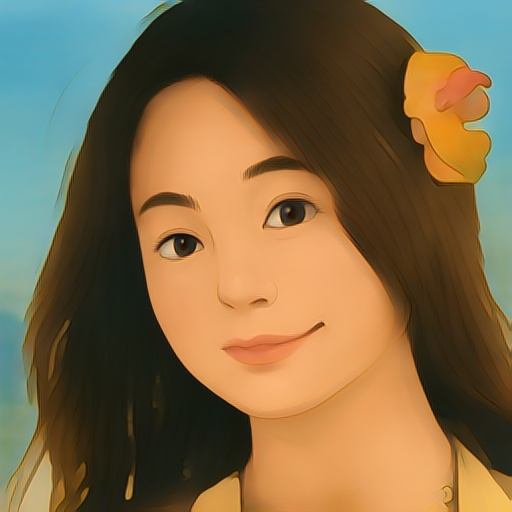
\includegraphics[width=\textwidth]{figChap3/style_results/d1.jpg}\\
{\scriptsize (d) Face Mode}
\end{column}
\end{columns}

\vspace{0.1cm}

\begin{columns}
\begin{column}{0.24\textwidth}
\centering
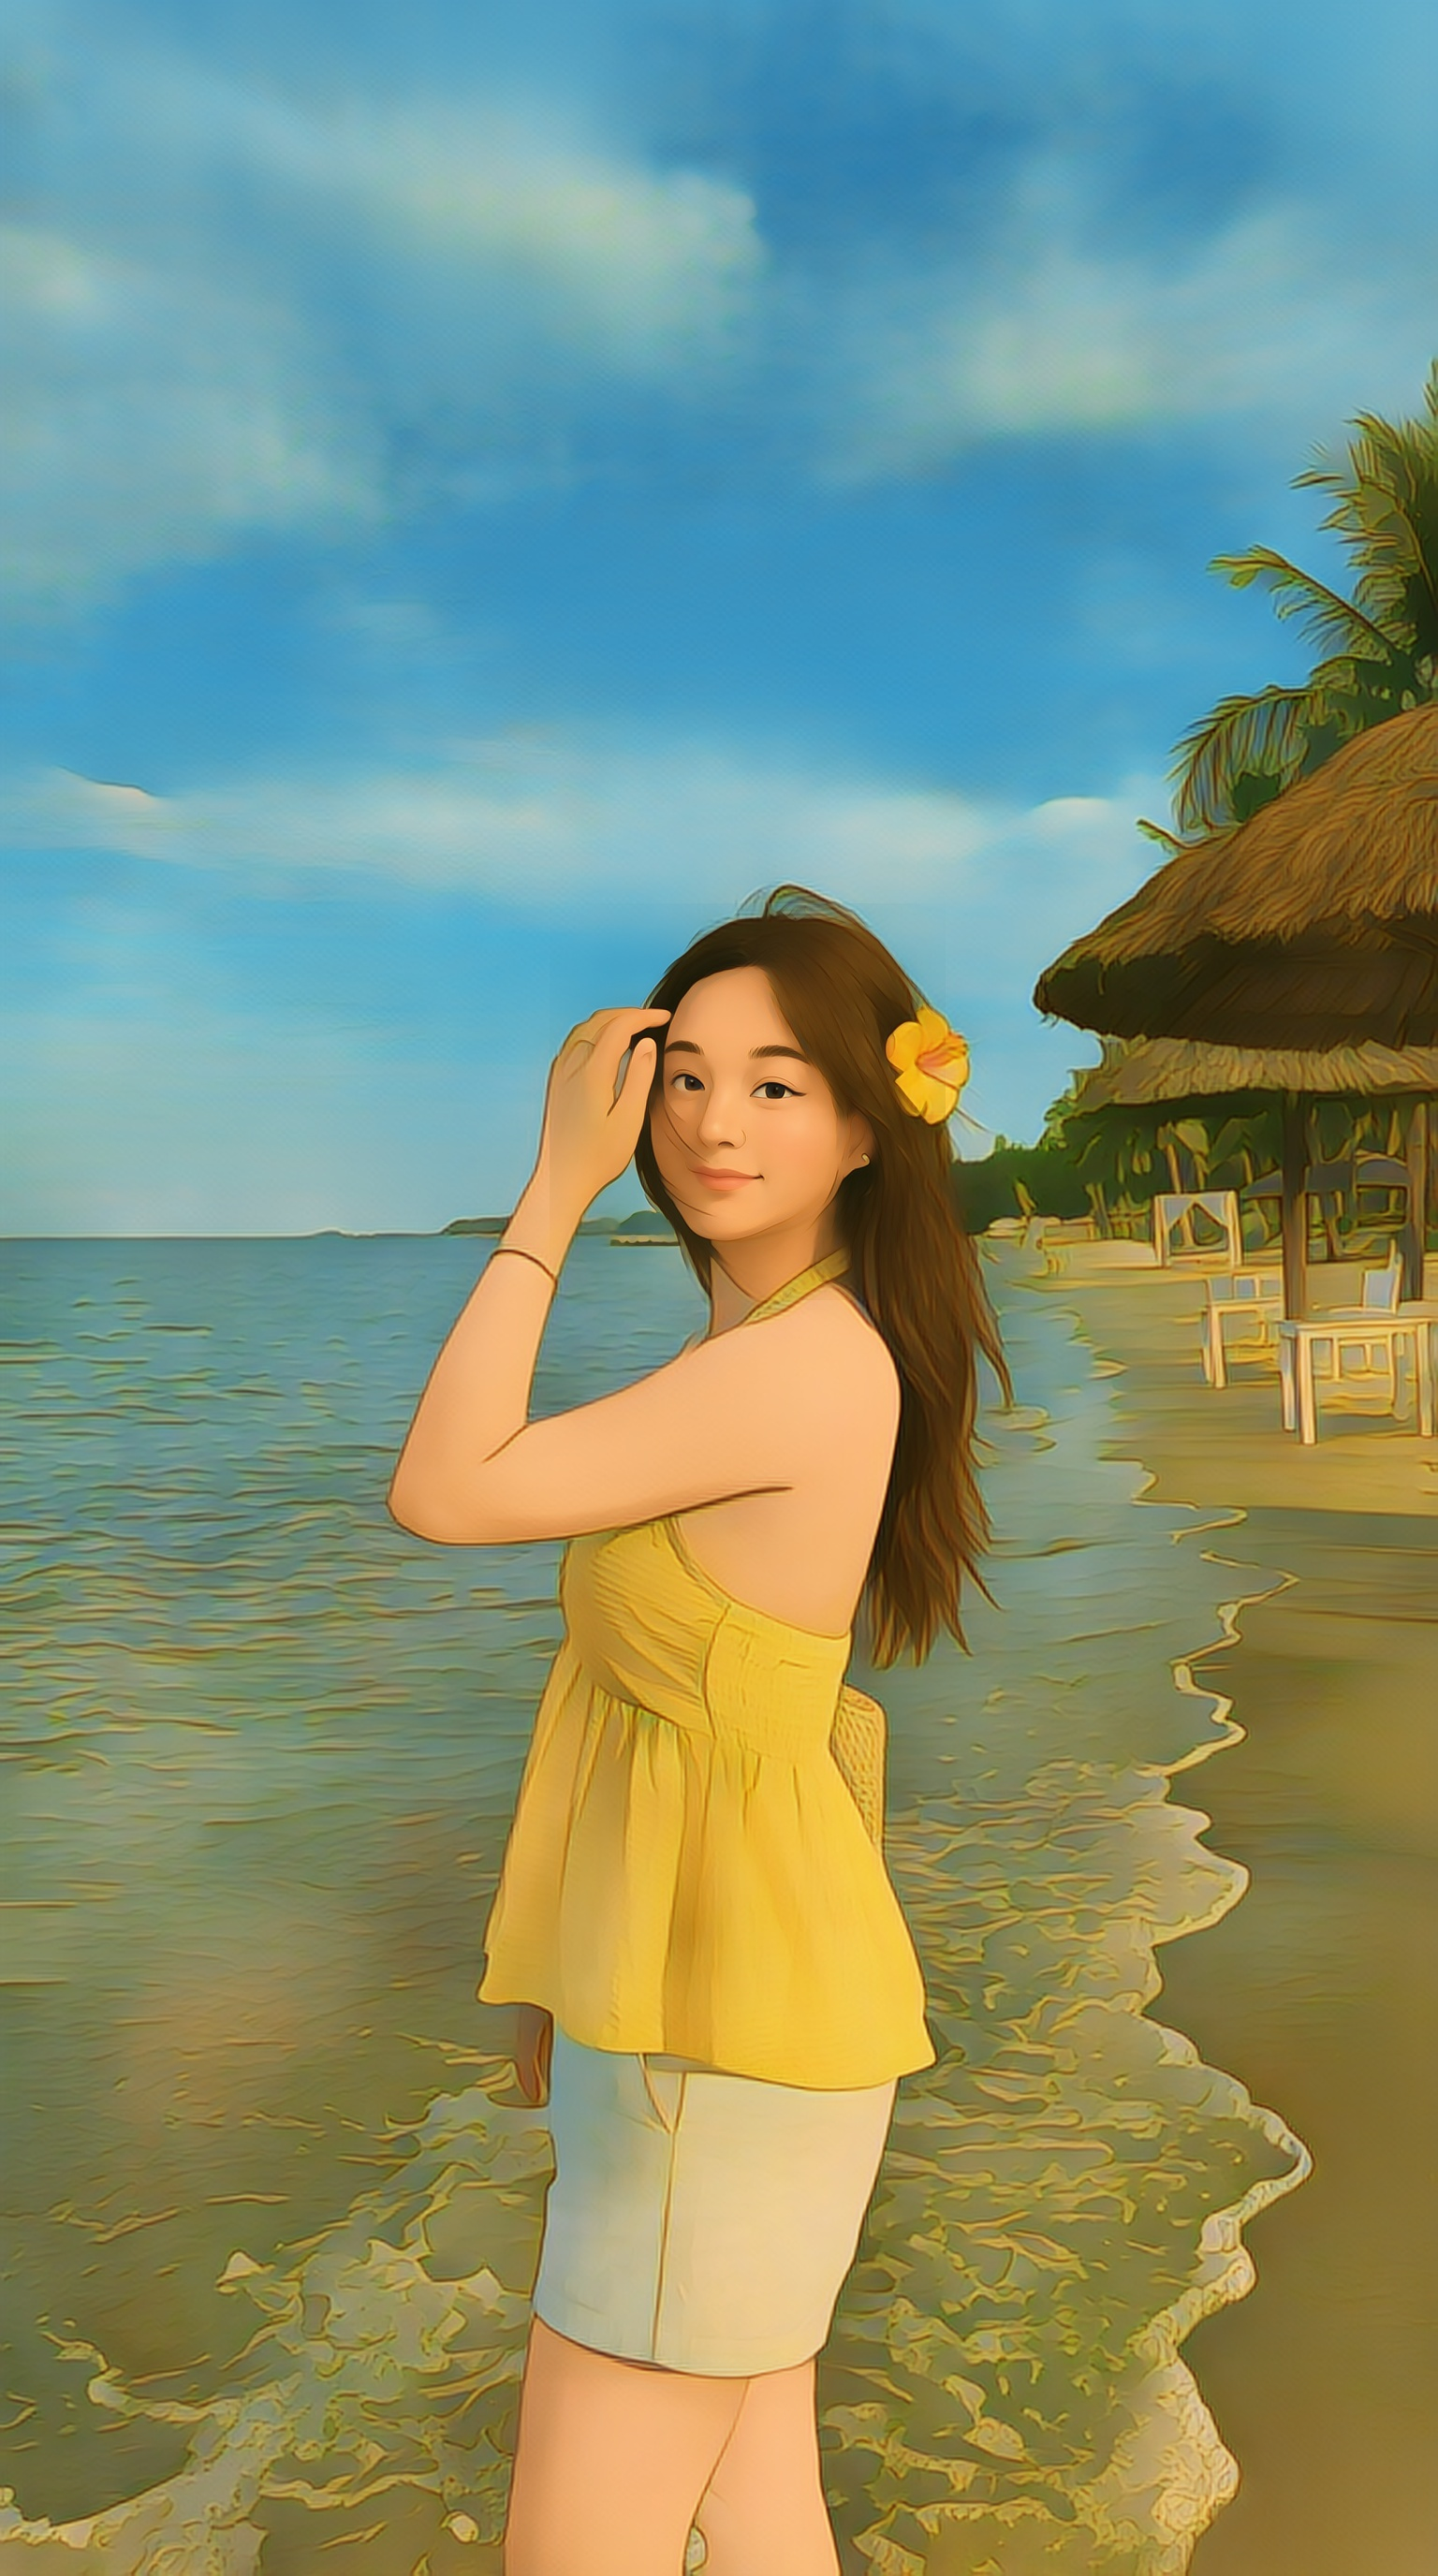
\includegraphics[width=\textwidth]{figChap3/style_results/e3.jpg}\\
{\scriptsize (a) Hybrid}
\end{column}
\begin{column}{0.24\textwidth}
\centering
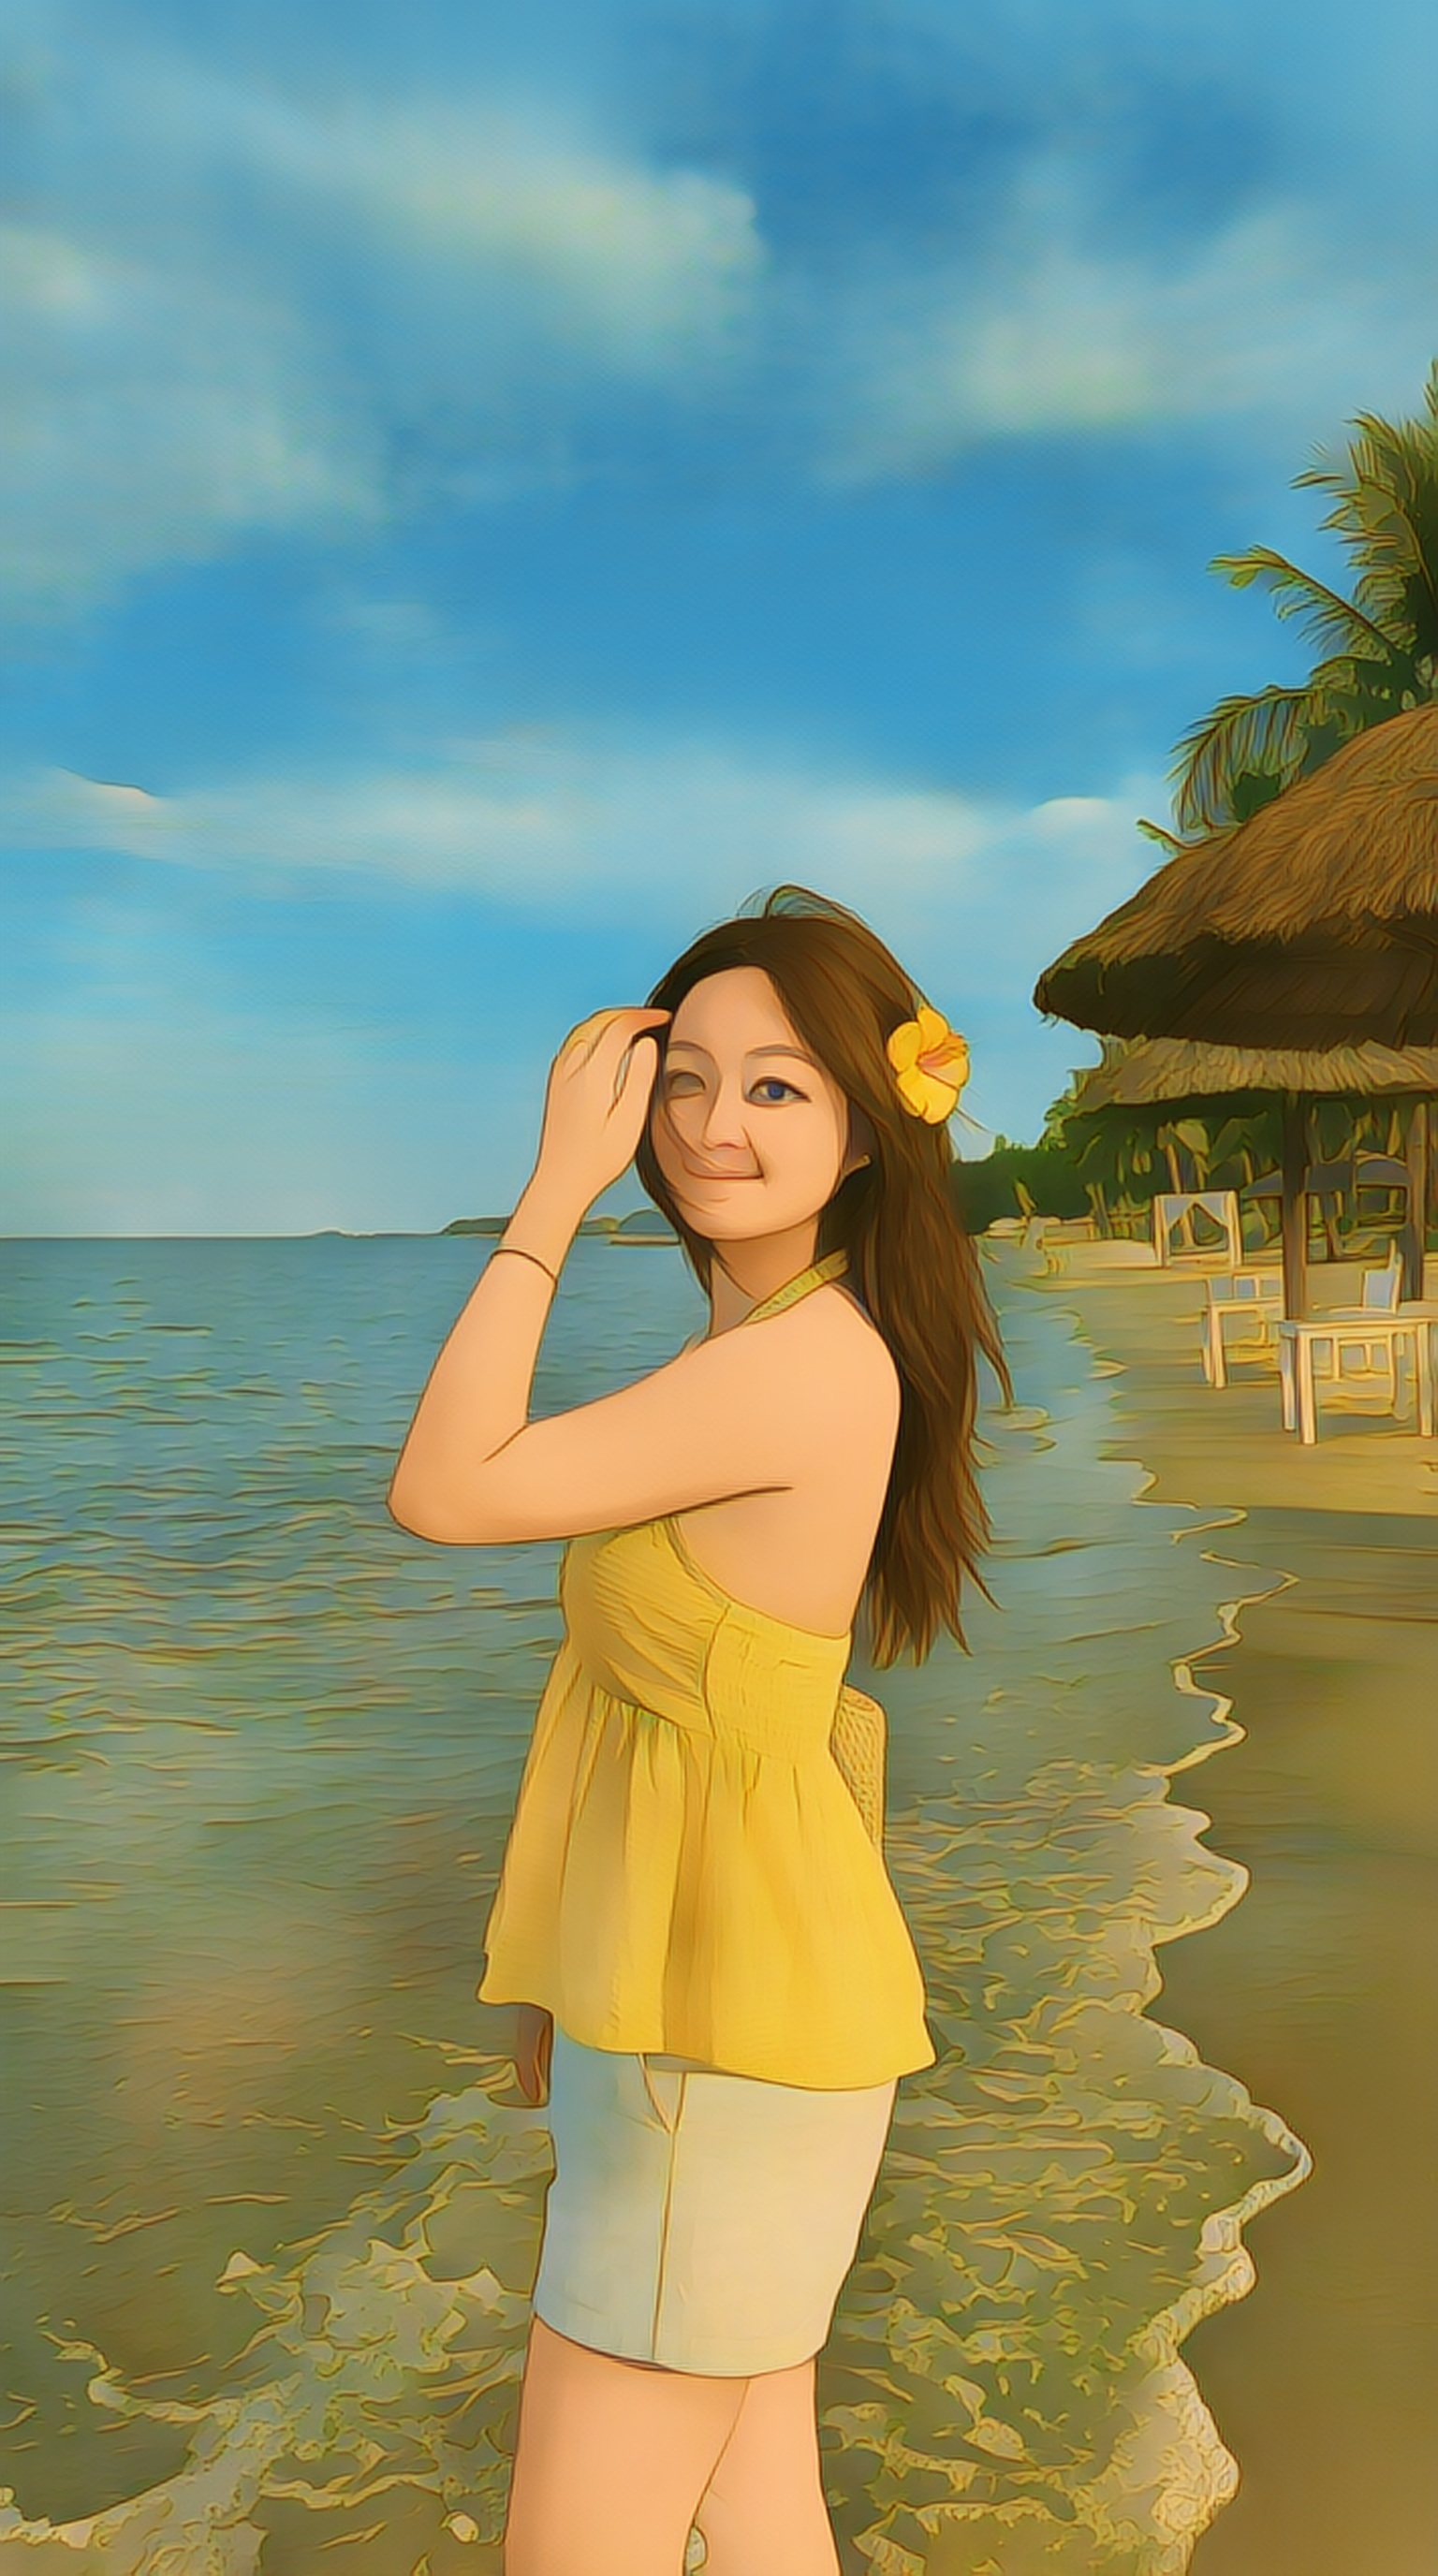
\includegraphics[width=\textwidth]{figChap3/style_results/b3.jpg}\\
{\scriptsize (b) Landscape}
\end{column}
\begin{column}{0.24\textwidth}
\centering

\includegraphics[width=\textwidth]{figChap3/style_results/c3.png}\\
{\scriptsize (c) Cắt mặt từ (b)}
\end{column}
\begin{column}{0.24\textwidth}
\centering
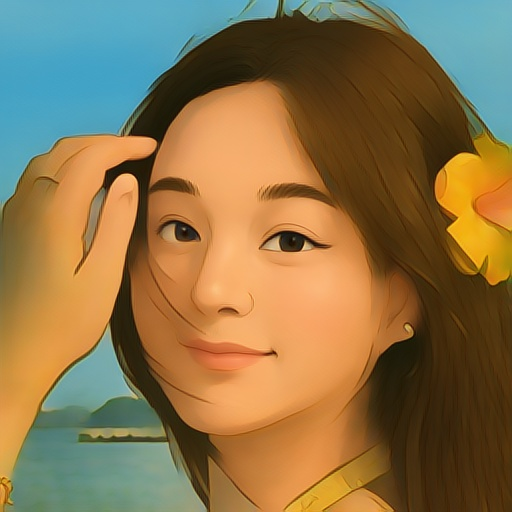
\includegraphics[width=\textwidth]{figChap3/style_results/d3.jpg}\\
{\scriptsize (d) Face Mode}
\end{column}
\end{columns}

\vspace{0.15cm}
{\small \textbf{Nhận xét:} Face Mode (d) sắc nét nhất cho khuôn mặt. Hybrid Mode (a) kết hợp tốt nền + mặt.}
\end{frame}

% --- Slide: Đánh giá Face Mode ---
\begin{frame}{Đánh giá Module Face Mode}
\begin{columns}[T]
\begin{column}{0.48\textwidth}
\textbf{Độ chính xác phát hiện khuôn mặt:}
\vspace{0.1cm}

\small
\begin{tabular}{lcc}
\toprule
\textbf{Kịch bản} & \textbf{Prec.} & \textbf{Recall} \\
\midrule
Trực diện, sáng tốt & 98.4\% & 97.1\% \\
Nghiêng $<30°$ & 94.2\% & 91.8\% \\
Nghiêng $30°$--$60°$ & 82.7\% & 76.3\% \\
Ánh sáng yếu & 88.1\% & 83.5\% \\
Mặt nhỏ $<32$px & 71.4\% & 65.9\% \\
\bottomrule
\end{tabular}
\end{column}
\begin{column}{0.48\textwidth}
\textbf{Phân tích tham số margin:}
\vspace{0.1cm}

\small
\begin{tabular}{cccl}
\toprule
\textbf{margin} & \textbf{FID} & \textbf{LPIPS} & \textbf{Nhận xét} \\
\midrule
0.3 & 63.1 & 0.401 & Cắt mất tóc \\
\rowcolor{lightblue} \textbf{0.5} & \textbf{58.6} & \textbf{0.384} & \textbf{Tối ưu} \\
0.7 & 61.3 & 0.396 & Thừa nền \\
\bottomrule
\end{tabular}

\vspace{0.3cm}
\begin{exampleblock}{Kết luận}
\small
\textbf{margin = 0.5} tối ưu cả FID, LPIPS lẫn chất lượng thị giác
\end{exampleblock}
\end{column}
\end{columns}
\end{frame}

% ============================================================================
% CHƯƠNG 5
% ============================================================================
\section{Kết luận và Hướng phát triển}

% --- Slide: Kết luận ---
\begin{frame}{Kết luận}
\begin{enumerate}
    \item \textbf{Phân tích kiến trúc DTGAN:} Double-Tail Generator, LADE, External Attention v3, 7 hàm mất mát chuyên biệt

    \item \textbf{Xây dựng pipeline Face Extraction} (đóng góp nguyên bản): RetinaFace + Margin Expansion, 3 chế độ (Face/Landscape/Hybrid), graceful degradation

    \item \textbf{Huấn luyện hội tụ ổn định:} 5 epoch pre-training + 69 epoch adversarial, không mode collapse

    \item \textbf{Kết quả vượt trội:}
    \begin{itemize}
        \item FID = \textbf{58.6}, LPIPS = \textbf{0.384} (Face Mode) — tốt nhất so với baseline
        \item Face Mode cải thiện $\sim$\textbf{8.7\%} FID so với Landscape
        \item Model ONNX \textbf{9.1 MB}, tốc độ \textbf{42 FPS} @ $256\times256$ GPU
    \end{itemize}

    \item \textbf{Ứng dụng web hoàn chỉnh:} React + FastAPI, hỗ trợ ảnh và video
\end{enumerate}
\end{frame}

% --- Slide: Mức độ hoàn thành ---
\begin{frame}{Mức độ hoàn thành mục tiêu}
\begin{table}
\centering
\small
\begin{tabular}{p{6.5cm}cp{4cm}}
\toprule
\textbf{Mục tiêu} & \textbf{Kết quả} & \textbf{Minh chứng} \\
\midrule
Nghiên cứu lý thuyết CNN, GAN, RetinaFace & \textcolor{resultgreen}{\checkmark} & Chương 1 \\
\midrule
Phân tích kiến trúc DTGAN & \textcolor{resultgreen}{\checkmark} & Chương 2 \\
\midrule
Xây dựng pipeline Face Extraction & \textcolor{resultgreen}{\checkmark} & Chương 3 (FID $\uparrow$8.7\%) \\
\midrule
Huấn luyện và đánh giá mô hình & \textcolor{resultgreen}{\checkmark} & Chương 4 (FID 58.6) \\
\midrule
Xây dựng ứng dụng demo & \textcolor{resultgreen}{\checkmark} & Web React + FastAPI \\
\bottomrule
\end{tabular}
\end{table}

\vspace{0.3cm}
\centering
\textbf{$\Rightarrow$ Tất cả 5/5 mục tiêu đã được hoàn thành đầy đủ}
\end{frame}

% --- Slide: Hạn chế và Hướng phát triển ---
\begin{frame}{Hạn chế và Hướng phát triển}
\begin{columns}[T]
\begin{column}{0.48\textwidth}
\begin{alertblock}{Hạn chế}
\small
\begin{itemize}
    \item Phụ thuộc tập dữ liệu huấn luyện
    \item RetinaFace giảm hiệu năng ở góc nghiêng $>60°$
    \item Chưa có temporal consistency cho video
    \item Hybrid Mode chậm khi $N > 5$ mặt
    \item CPU chỉ $\sim$1.1 FPS @ $512^2$
\end{itemize}
\end{alertblock}
\end{column}
\begin{column}{0.48\textwidth}
\begin{exampleblock}{Hướng phát triển}
\small
\begin{itemize}
    \item \textbf{Face Alignment:} Khai thác 5 landmarks để căn chỉnh mặt
    \item \textbf{Poisson Blending:} Thay feathered blending
    \item \textbf{Temporal consistency:} Optical flow cho video
    \item \textbf{Multi-style:} Nội suy tham số LADE
    \item \textbf{Mobile:} TFLite/CoreML + INT8 quantization
\end{itemize}
\end{exampleblock}
\end{column}
\end{columns}
\end{frame}

% ============================================================================
% SLIDE KẾT THÚC
% ============================================================================
{
\setbeamertemplate{footline}{}
\begin{frame}
\vfill
\centering
\begin{beamercolorbox}[sep=12pt,center,shadow=true,rounded=true]{title}
{\Large \textbf{CẢM ƠN QUÝ THẦY CÔ VÀ HỘI ĐỒNG\\[0.3cm] ĐÃ LẮNG NGHE!}}
\end{beamercolorbox}

\vspace{0.8cm}

{\large Nguyễn Trọng Nhân --- 24025149}\\[0.2cm]
{\normalsize GVHD: TS. Ma Thị Châu}\\[0.2cm]
{\normalsize Trường Đại học Công nghệ --- ĐHQGHN}\\[0.5cm]

{\normalsize \textit{Hà Nội, 2026}}

\vfill
\end{frame}
}

\end{document}
